% ============================================================
% 整合导言区：国赛格式 + 算法/假设环境 + Draft 提速开关
% 编译方式: latexmk -xelatex
% ============================================================

% ---------- 草稿模式开关 ----------
%\def\FASTDRAFT{}

\ifdefined\FASTDRAFT
  \documentclass[draft,12pt,a4paper]{ctexart}
\else
  \documentclass[fontset=windows,12pt,a4paper]{ctexart}
\fi

% ---------- 页面几何 ----------
\usepackage{geometry}
\geometry{
    paperwidth=210mm, paperheight=297mm,
    left=2.5cm, right=2.5cm,
    top=2.5cm, bottom=2.5cm
}

% ---------- 数学 ----------
\usepackage{amsmath,amsfonts,amssymb,bm,amsthm}

% ---------- 图片与颜色 ----------
\ifdefined\FASTDRAFT
  \usepackage[draft]{graphicx}
\else
  \usepackage{graphicx}
  \DeclareGraphicsExtensions{.pdf,.png,.jpg,.jpeg}
\fi
\usepackage{xcolor}

% ---------- 子图 ----------
\usepackage{subcaption}

% ---------- 表格 ----------
\usepackage{booktabs,tabularx,multirow,array,longtable,colortbl}
\renewcommand{\heavyrulewidth}{2.25pt}
\renewcommand{\lightrulewidth}{0.75pt}
\renewcommand{\cmidrulewidth}{0.75pt}
\renewcommand{\arraystretch}{1.25}

% ---------- 浮动体 ----------
\usepackage{float}

% ---------- 列表 ----------
\usepackage[shortlabels]{enumitem}
\setlist{nosep,leftmargin=1.5em}

% ---------- 算法与代码 ----------
\usepackage{algorithm}
\usepackage{algpseudocode}
\floatname{algorithm}{算法}
\renewcommand{\algorithmicrequire}{\textbf{输入：}}
\renewcommand{\algorithmicensure}{\textbf{输出：}}

\usepackage{listings}
\lstset{
    language=Python,
    basicstyle=\small\ttfamily,
    keywordstyle=\color{blue}\bfseries,
    commentstyle=\color{green!50!black}\itshape,
    stringstyle=\color{orange},
    numbers=left,
    numberstyle=\tiny\color{gray},
    stepnumber=1,
    numbersep=8pt,
    backgroundcolor=\color{gray!10},
    frame=single,
    frameround=tttt,
    breaklines=true,
    showstringspaces=false,
    tabsize=4,
    captionpos=b,
    xleftmargin=2em,
    xrightmargin=1em,
    aboveskip=1em,
    belowskip=1em
}

% ---------- 页眉页脚 ----------
\usepackage{fancyhdr,lastpage}
\pagestyle{fancy}
\fancyhf{}
\fancyfoot[C]{\thepage}
\renewcommand{\headrulewidth}{0pt}

% ---------- 标题格式 ----------
\ctexset{
    section = {
        number = \chinese{section}、,
        format = \zihao{3}\heiti\bfseries\centering,
        beforeskip = 1.0ex plus 0.5ex minus 0.2ex,
        afterskip  = 1.0ex plus 0.5ex minus 0.2ex
    },
    subsection = {
        format = \zihao{4}\heiti\bfseries\raggedright,
        beforeskip = 0.8ex plus 0.3ex minus 0.1ex,
        afterskip  = 0.8ex plus 0.3ex minus 0.1ex
    },
    subsubsection = {
        format = \zihao{-4}\heiti\bfseries\raggedright,
        beforeskip = 0.5ex plus 0.2ex minus 0.1ex,
        afterskip  = 0.5ex plus 0.2ex minus 0.1ex
    }
}

% ---------- 图表标题格式 ----------
\usepackage{caption}
\captionsetup[figure]{labelsep=space, font=small}
\captionsetup[table]{labelsep=space, font=small}

% ---------- 行距 ----------
\usepackage{setspace}
\setstretch{1.25}

% ---------- 数学定理环境 ----------
\theoremstyle{definition}
\newtheorem{definition}{定义}[section]
\newtheorem{theorem}{定理}[section]
\newtheorem{lemma}{引理}[section]
\newtheorem{assumption}{假设}[section]

% ---------- 绘图 ----------
\usepackage{tikz}
\usetikzlibrary{shapes.geometric, arrows.meta, positioning, calc}
\usepackage{pgfplots}
\pgfplotsset{compat=1.18}

\ifdefined\FASTDRAFT
\else
  \usetikzlibrary{external}
  \tikzexternalize[prefix=tikz-cache/]
\fi

% ---------- 超链接 ----------
\ifdefined\FASTDRAFT
  \usepackage[draft,hidelinks,bookmarks=false,unicode=true]{hyperref}
\else
  \usepackage[hidelinks,bookmarks=true,bookmarksnumbered=true,unicode=true]{hyperref}
\fi
\usepackage{cleveref}

% ---------- 自定义命令 ----------
\newcommand{\diff}{\mathrm{d}}
\newcommand{\E}{\mathrm{E}}
\DeclareMathOperator*{\argmin}{arg\,min}
\DeclareMathOperator*{\argmax}{arg\,max}

% ============================================================
% 正文开始
% ============================================================
\begin{document}

\newcommand{\keywords}[1]{\par\vspace{6pt}\noindent\textbf{关键词：#1}\par}
\renewcommand{\lstlistingname}{代码}

%================ 首页 =================
\begin{center}
  {\zihao{3}\bfseries 基于\textbf{对角线代表性窄条与分段ABD柔度串联模型}的芯片封装\textbf{等效热弹性参数}估计\par}
\end{center}

%================ 摘要 =================
\begin{center}
  {\zihao{4}\bfseries \textbf{摘\quad 要}}
\end{center}
\vspace{0.1cm}

芯片集成度持续攀升，单块PCBA上电子元件愈发密集，反复的温度循环与机械冲击等服役工况均会导致封装元件与PCB板之间焊料的疲劳与失效，而封装角点因热失配位移累积最大，通常成为失效风险最高的位置。因此，在封装设计早期阶段准确估计角点沿对角线方向的\textbf{等效拉伸杨氏模量}、\textbf{等效弯曲杨氏模量}和\textbf{等效热膨胀系数}，对于预判焊料疲劳寿命、优化封装结构具有直接的工程意义。

针对问题一，我们考虑到BGA封装在高低温循环工况下角点失效风险较高的实际背景，将PCBA模型抽象为沿封装对角线方向的\textbf{非均质弹性板}。我们建立了\textbf{对角线代表性窄条与三层变换截面模型}，利用\textbf{面积均匀化方法}将离散焊球阵列折算为等效中间层，采用\textbf{层合板理论中的轴向刚度与弯曲刚度分解思路}，分别推导了沿对角线方向的\textbf{等效拉伸杨氏模量}、\textbf{等效弯曲杨氏模量}以及\textbf{等效热膨胀系数}的显式表达式。我们给出了完整的计算流程与\textbf{参数补齐规则}，并通过\textbf{解析退化校验}验证了模型的自洽性。

针对问题二，在问题一的基础上，我们进一步处理QFN封装沿中心至角点半对角线方向的等效参数估计问题。QFN本体为三层分区结构，其中芯片、铜焊盘和局部焊料仅占据部分对角线路径，因此局部截面随路径坐标变化。我们构建了\textbf{分段局部标量ABD模型}，先计算各段截面的拉伸刚度、耦合刚度和弯曲刚度，再沿半对角线路径按\textbf{柔度串联}串联得到等效ABD矩阵。通过三个单位工况分别定义了QFN的\textbf{等效拉伸杨氏模量}、\textbf{等效弯曲杨氏模量}和\textbf{等效热膨胀系数}。

针对问题三，我们处理实际BGA封装在角点缺球缺陷下的等效参数估计问题。我们建立了带角点窗口的\textbf{三区段ABD柔度等效模型}，用\textbf{等效柔度截面积}标定单个焊球的剪切刚度，将437个离散焊球折算为连续连接层，并在角点设置与对角线路径对齐的\textbf{窗口区段}，按窗口内实际球数局部折算连接层模量，使缺球位置直接进入整体等效参数。计算得到437阵列沿对角线方向的等效拉伸杨氏模量30.80 GPa、等效弯曲杨氏模量22.85 GPa、等效热膨胀系数19.28 ppm/K；同时构建\textbf{二维壳-离散弹簧校核模型}，从整体能量、角点相对位移和最近焊球载荷三个层面检验均匀化主模型的适用范围，结果表明437阵列相对441阵列的角点缺球本身引起的整体参数变化不足0.2\%，而角点相对位移上升5.78\%，整体量与局部量需要分层评价。

我们围绕BGA与QFN两类主流封装，建立了基于\textbf{对角线代表性窄条}的\textbf{等效热弹性参数估计体系}。三问模型逻辑递进，逐步扩展与修正，力学口径一致，由简至繁逐步扩展，并辅以\textbf{解析退化校验}与\textbf{二维离散校核}，为芯片封装早期设计阶段的可靠性评估提供了简便、快速且可量化的计算框架。

\noindent\textbf{关键词：}\textbf{BGA封装}; \textbf{等效热弹性参数}; \textbf{变换截面法}; \textbf{分段ABD柔度串联}; \textbf{角点窗口}
\newpage

%================ 1 问题重述 =================
\section{问题重述}
\subsection{问题背景}

BGA和QFN封装技术因其高引脚密度和优良的电学性能，已成为现代高性能芯片与印刷电路板互连的主流方案。在服役过程中，封装组件需要经受高低温循环、功率循环及机械振动等多种载荷作用，其中温度循环是导致焊料互连失效的最主要因素之一$^{\textbf{[\ref{ref:4}]}}$。由于PCB、焊球和封装层三者的热膨胀系数存在显著差异，温度变化会在层间界面附近诱发热失配应力与应变。经过足够多次循环后，焊料将发生累积塑性变形并最终形成疲劳裂纹，导致电气开路或功能丧失。因此，在封装设计的早期阶段，准确估计关键位置处的等效力学参数和热膨胀参数，对于预判焊料疲劳寿命、优化封装结构具有直接的工程价值。


\subsection{问题的提出}

我们需解决以下三个问题。

问题一：针对BGA封装PCB-焊球-BGA三层连续结构，将PCBA模型视作为非均质的弹性板，估计红圈角点位置沿对角线方向的\textbf{等效拉伸杨氏模量}、\textbf{等效弯曲杨氏模量}和\textbf{等效热膨胀系数}。

问题二：在问题一的基础上，将建模对象从BGA的简单三层连续结构拓展到QFN的三层分区结构。由于芯片、铜焊盘和局部焊料仅占据部分对角线路径，局部截面随路径坐标变化，估计QFN封装在角点位置沿对角线方向的\textbf{等效拉伸杨氏模量}、\textbf{等效弯曲杨氏模量}和\textbf{等效热膨胀系数}。

问题三：问题一是简化的BGA封装，实际情况下，BGA的焊球分布会存在缺陷。实际阵列存在中心空隙、外环结构和四个最外角位置无球。试利用数学模型并结合仿真计算，估计实际BGA封装在角点位置沿对角线方向的\textbf{等效杨氏模量}和\textbf{等效热膨胀系数}。

%================ 2 问题分析 =================

\section{问题分析}

我们的总体分析思路如下：首先明确三个问题所求的\textbf{三个等效参数}的工程含义与所需信息; 随后建立基于\textbf{代表性窄条}的简化力学模型，利用\textbf{层合板理论}$^{\textbf{[\ref{ref:3}]}}$推导显式公式。

问题一属于\textbf{等效物理参数估计问题}。核心在于如何将PCB、焊球阵列和BGA封装这三层非均质结构，简化为一个沿对角线方向具有等效刚度与等效\textbf{热膨胀系数}的均匀窄条。考虑到题目仅给出杨氏模量和热膨胀系数，未给出泊松比，我们拟采用\textbf{一维窄条模型}，在不虚构额外材料参数的前提下完成一阶估计。具体地，我们先用两个红圈角点确定对角线方向，再沿该方向截取单位宽度\textbf{代表性窄条}; 对离散焊球阵列采用\textbf{面积均匀化思想}折算为等效中间层; 最后基于\textbf{变换截面法}分别计算\textbf{拉伸刚度}、\textbf{弹性中性轴}、弯曲刚度和\textbf{热膨胀系数}。

问题二同样属于\textbf{等效物理参数估计问题}，但建模对象从BGA的简单三层结构扩展为QFN的三层分区结构。由于芯片、铜盘和焊料仅占据部分对角线路径，局部截面随路径坐标变化，因此不能沿用问题一的固定截面思路。我们拟采用\textbf{分段局部标量ABD模型}：先根据芯片、铜盘和焊料的几何边界将半对角线路径分为若干段，对每一段建立局部拉伸、耦合和弯曲刚度; 再沿路径按\textbf{柔度串联}串联得到等效ABD矩阵; 最后通过三个单位工况分别定义\textbf{等效拉伸杨氏模量}、\textbf{等效弯曲杨氏模量}和\textbf{等效热膨胀系数}。该思路直接继承问题一的力学口径，但在建模尺度上做了结构性扩展。

问题三属于\textbf{带缺陷实际结构的等效参数估计与仿真验证问题}。与问题一的理想满布阵列不同，实际BGA阵列存在中心空隙、外环结构和角点缺球，全局均匀化会抹去缺球的位置信息，而题目又明确要求结合仿真计算。我们拟建立\textbf{角点窗口三区段ABD柔度等效模型}作为主模型：先用\textbf{等效柔度截面积}标定单个焊球的剪切刚度，再将离散连接器折算为连续连接层; 在角点设置与对角线路径对齐的\textbf{窗口区段}，按窗口内实际球数局部折算连接层模量，使缺球直接进入整体等效参数; 同时建立\textbf{二维壳-离散弹簧模型}作为验证层，分别考察整体能量、角点相对位移和最近焊球载荷，并辅以窗口宽度与材料参数的灵敏度分析。该思路是问题一均匀化思想和问题二分段串联思想在具体几何缺陷场景下的结合。

三问采用统一的对角线窄条力学口径，并统一采用三类标准单位工况定义三个等效参数：单位中性轴拉伸工况（$\Delta T=0,\kappa=0,N\neq0$）定义等效拉伸杨氏模量；单位纯弯曲工况（$\Delta T=0,\varepsilon_n=0,M_n\neq0$）定义等效弯曲杨氏模量；自由热膨胀工况（$\Delta T\neq0,N=0,M_n=0$）定义等效热膨胀系数，并以自由热曲率$\kappa_T$作为辅助输出。

下图展示了我们全文的处理流程。
\begin{figure}[H]
  \centering
  \includegraphics[width=1\textwidth]{output/figs/流程图.png}
  \caption{全文技术路线图}\label{fig:flow_chart}
\end{figure}

%================ 3 模型假设 =================
\newpage
\section{模型假设}

\textbf{1. 温度与材料线性：}温度变化为准静态过程，同一厚度截面内温度近似均匀; 三种材料处于小变形线弹性热弹性范围，材料参数在所讨论温区内近似为常数。

\textbf{2. 层间连续与界面理想：}PCB层和BGA层在所取窄条内连续; 层间界面在失效前保持理想结合，位移连续。

\textbf{3. 标量ABD简化：}沿对角线方向截取单位宽度代表性窄条，因题目未给出泊松比，我们采用标量ABD模型，不虚构完整二维本构矩阵或未给出的各向异性参数。

\textbf{4. 窄条简化：}沿对角线方向截取单位宽度\textbf{代表性窄条}，采用\textbf{Kirchhoff-Love薄板假设}的一维形式，即截面应变沿厚度方向呈线性分布。

\textbf{5. 参数给定与模型适用范围：}题目给定的$E_1$默认已经代表PCB沿对角线方向的有效模量; 暂不考虑底充胶、焊料蠕变、界面脱粘和应力集中; 我们模型仅估计整体等效参数，不预测局部峰值应力、蠕变、脱层或疲劳寿命。


%================ 4 问题一 =================
\section{问题一：PCBA\textbf{非均质弹性板}的\textbf{等效热弹性参数}估计}

在高低温循环工况下，PCB、焊球阵列和BGA封装由于材料热膨胀系数不同，会在界面附近产生\textbf{热失配变形}。BGA封装角点距离封装中心最远，热失配位移沿对角线方向逐步累积，同时角部又受到自由边缘和离散焊球布置的影响，因此角点通常成为失效风险较高的位置。题目要求我们估计红圈角点沿封装对角线方向的\textbf{等效拉伸杨氏模量}、\textbf{等效弯曲杨氏模量}和\textbf{等效热膨胀系数}。我们的初步思路是先用题图中两个红圈角点确定封装的对角线方向，再沿该方向截取一个\textbf{代表性窄条}，把PCB、焊球阵列和BGA分别处理为三层材料。PCB层和BGA层是连续层，焊球阵列层则不是连续材料，因此我们先用焊球\textbf{有效面积占比}把离散焊球折算为等效中间层，再采用层合结构中的\textbf{变换截面思想}，分别计算\textbf{拉伸刚度}、\textbf{弹性中性轴}、弯曲刚度和\textbf{热膨胀系数}。需要说明的是，这种均匀化模型会忽略红圈角点与封装内部、对角线中部之间的平面位置差异; 红圈角点在这里用于定义计算方向和代表性截面，而不是被解析为一个具有独立局部参数的平面坐标点。

我们考虑到\textbf{Mori Tanaka方法}$^{\textbf{[\ref{ref:6}]}}$适用于夹杂嵌入连续基体的复合材料，而本题中间层是孤立焊球与空气间隙，空气刚度近似为零，不能提供连续基体约束,因此没有选择为主模型。\textbf{Hashin与Shtrikman界限}$^{\textbf{[\ref{ref:7}]}}$可以估计多相材料有效弹性模量的允许范围，但本题的关键几何信息是层序、厚度、层中心距和焊球面积占比，直接使用该界限会过宽，因此它更适合作为结果合理性检查，而不适合作为主求解方法。基于这些考虑，我们最终采用\textbf{对角线代表性窄条加三层变换截面模型}作为问题一的基线方案。

问题一涉及的主要符号如下表所示。

\begin{table}[H]\centering
  \caption{问题一主要符号说明}\label{tab:symbol-q1}
  \small
  \begin{tabular}{ccc}
    \toprule
    符号 & 说明 & 单位 \\
    \midrule
    $E_1$ & PCB层杨氏模量 & Pa \\
    $E_2$ & 单个焊球材料杨氏模量 & Pa \\
    $E_3$ & BGA封装层杨氏模量 & Pa \\
    $\alpha_1$ & PCB层热膨胀系数，等于$CTE_1$ & 1/K \\
    $\alpha_2$ & 焊球材料热膨胀系数，等于$CTE_2$ & 1/K \\
    $\alpha_3$ & BGA层热膨胀系数，等于$CTE_3$ & 1/K \\
    $L$ & BGA封装边长 & m \\
    $m$ & 单方向焊球数量，总数量为$m^2$ & 无量纲 \\
    $h_1,h_2,h_3$ & PCB层、焊球层和BGA层厚度 & m \\
    $h$ & 三层总厚度 & m \\
    $\phi$ & 焊球层有效面积占比 & $0 \leq \phi \leq 1$ \\
    $\chi_i$ & 第$i$层折算系数 & 无量纲 \\
    $q_i$ & 第$i$层折算模量，$q_i=\chi_i E_i$ & Pa \\
    $z_n$ & 弹性中性轴坐标 & m \\
    $S_0$ & 单位宽度截面轴向刚度系数 & N/m \\
    $J$ & 关于弹性中性轴的弯曲刚度系数 & N$\cdot$m \\
    $E_{d,t}$ & 沿对角线方向等效拉伸杨氏模量 & Pa \\
    $E_{d,b}$ & 沿对角线方向等效弯曲杨氏模量 & Pa \\
    $\alpha_d$ & 沿对角线方向等效热膨胀系数 & 1/K \\
    \bottomrule
  \end{tabular}
\end{table}

题图中的两个红圈角点位于正方形封装的一条对角线两端。以封装中心为原点，对角线方向单位向量及路径范围为
\begin{equation}\label{eq:diagonal}
\mathbf e_d:=\frac{1}{\sqrt 2}(1,1),
\qquad 0\le s\le\sqrt 2L.
\end{equation}

式中，$s$ 为平面内路径坐标，不能与厚度方向坐标 $z$ 混用。均匀化后所得参数不随 $s$ 改变，红圈角点仅用于确定研究方向。

我们沿$\mathbf e_d$截取一条单位宽度代表性窄条。该处理由题目条件和所求量共同决定,因为题目明确询问沿对角线方向的等效参数，窄条模型与该方向直接对应。并且，题目只给出杨氏模量和热膨胀系数，没有给出泊松比，窄条模型可以在不虚构泊松比的情况下完成一阶估计。层间并联承载、中性轴偏移和弯曲杠杆效应在模型中仍然保留。

\begin{figure}[H]
  \centering
  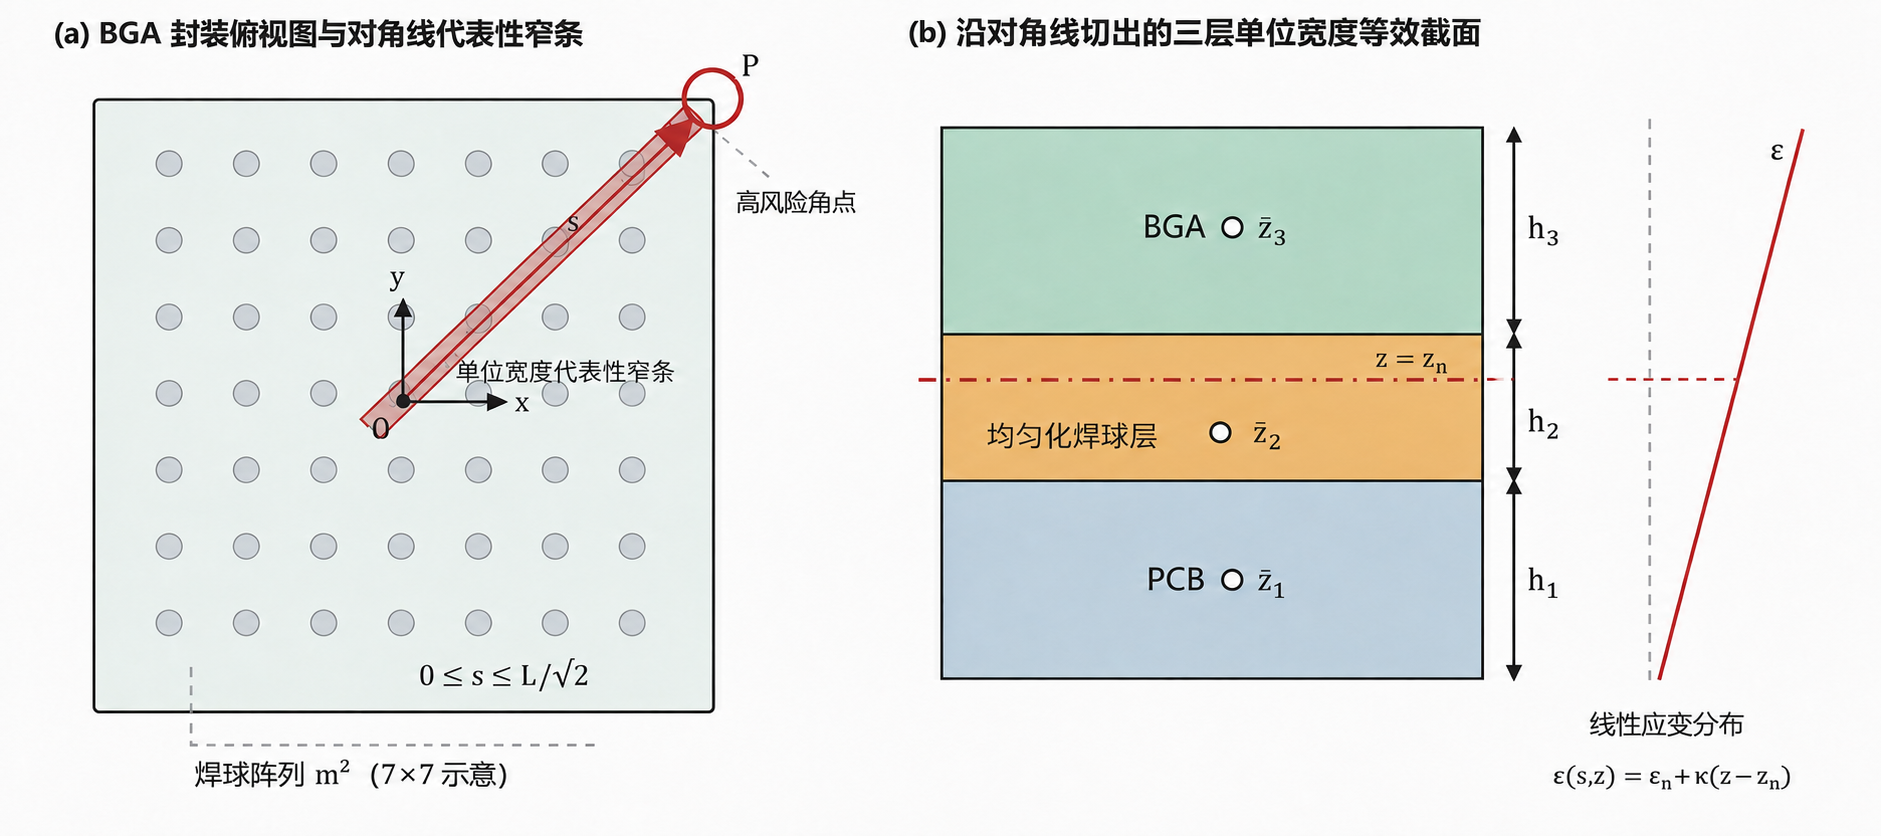
\includegraphics[width=0.95\textwidth]{output/figs/问题一对角线图.png}
  \caption{问题一：BGA封装对角线代表性窄条示意}\label{fig:q1-diagonal}
\end{figure}

图~\ref{fig:q1-diagonal}(a)给出BGA封装俯视图，红色窄条为从封装中心$O$沿对角线至高风险角点$P$的单位宽度代表性窄条，$s$为路径坐标；(b)给出沿对角线方向的截面分层示意。该图直观展示了本文三问统一采用的对角线窄条建模口径。

焊球没有填满整个中间层，空气间隙也不承担拉伸和弯曲载荷。设焊球为\textbf{圆柱体},单球有效承载面积为 $A_{b,\mathrm{eff}}$,据此折算离散的焊球层的贡献。
\begin{equation}\label{eq:phi}
\phi:=\frac{m^2A_{b,\mathrm{eff}}}{L^2},
\end{equation}

在理想界面和线弹性等效框架下，取$\chi_1=1,\quad \chi_2=\phi,\quad \chi_3=1$，对应的折算模量为
$
q_1:=E_1,\quad
 q_2:=\phi E_2,\quad
 q_3:=E_3.
$


在相同宏观应变下，承载面积按比例贡献轴力。从 PCB 底面起建立厚度坐标，三层形心为
$\bar z_1:=\frac{h_1}{2},\quad
 \bar z_2:=h_1+\frac{h_2}{2},\quad
 \bar z_3:=h_1+h_2+\frac{h_3}{2}.$


令 $z_n$ 为弹性中性轴坐标，$\varepsilon_n$ 为中性轴应变，$\kappa$ 为曲率。截面应变为
\begin{equation}\label{eq:strain-neutral}
\zeta:=z-z_n,
\qquad \varepsilon_d(z)=\varepsilon_n+\zeta\kappa.
\end{equation}

第 $i$ 层的一维热弹性本构为
\begin{equation}\label{eq:constitutive}
\sigma_i(z)=q_i\left[\varepsilon_n+(z-z_n)\kappa-\alpha_i\Delta T\right],
\qquad \alpha_i:=\mathrm{CTE}_i.
\end{equation}

单位宽度截面的轴力和弯矩为
\begin{equation}\label{eq:force-moment}
\frac Nb=\sum_{i=1}^{3}\int_{z_i^{(0)}}^{z_i^{(1)}}\sigma_i(z)\,\diff z,
\qquad
\frac Mb=\sum_{i=1}^{3}\int_{z_i^{(0)}}^{z_i^{(1)}}\sigma_i(z)(z-z_n)\,\diff z.
\end{equation}

定义轴向刚度系数和一阶刚度矩：
\begin{equation}\label{eq:S0}
S_0:=\sum_{i=1}^{3}q_ih_i,
\qquad
S_1:=\sum_{i=1}^{3}q_ih_i\bar z_i.
\end{equation}

选择 $z_n$ 使拉伸与弯曲的交叉刚度为零，则
\begin{equation}\label{eq:neutral}
0=\sum_{i=1}^{3}q_ih_i(\bar z_i-z_n)
=S_1-z_nS_0
\quad\Rightarrow\quad
\boxed{z_n=\frac{S_1}{S_0}}.
\end{equation}

由参数定义域可知 $S_0>0$，故式\eqref{eq:neutral}中的除法成立。

\subsection{求等效拉伸杨氏模量}

令 $\Delta T=0$ 且 $\kappa=0$。真实三层窄条与等效均质窄条在相同轴向应变下具有相同轴力：
\begin{equation}
\frac Nb
=\sum_{i=1}^{3}q_ih_i\varepsilon_n
=S_0\varepsilon_n
=E_{d,t}h\varepsilon_n.
\end{equation}

当 $\varepsilon_n\ne0$ 时，消去共同应变，得到
\begin{equation}\label{eq:Edt}
\boxed{
E_{d,t}=\frac{S_0}{h}
=\frac{E_1h_1+\phi E_2h_2+E_3h_3}{h_1+h_2+h_3}
}.
\end{equation}

式\eqref{eq:Edt}是等应变条件下的刚度—厚度加权结果，与 Voigt 均匀应变思想一致。从物理图像看，式\eqref{eq:Edt}是按刚度厚度加权，而不是简单按厚度加权。某一层的$E_i h_i$越大，它抵抗同一轴向应变的能力越强，对等效拉伸模量的贡献也越大。

\subsection{求等效弯曲杨氏模量}

对于单位宽度矩形窄条，第 $i$ 层绕自身形心轴的惯性矩系数为
\begin{equation}
I_{i,c}:=\frac{h_i^3}{12}.
\end{equation}

式中，下标 $c$ 表示形心轴。由于已取单位宽度，$I_{i,c}$ 的量纲为 $\mathrm{m}^3$；与折算模量 $q_i$ 相乘后，$q_iI_{i,c}$ 才是该层绕自身形心轴的弯曲刚度贡献。

由平行移轴定理，第 $i$ 层关于整体中性轴的几何积分为
\begin{equation}
\int_{z_i^{(0)}}^{z_i^{(1)}}(z-z_n)^2\,\diff z
=\frac{h_i^3}{12}+h_i(\bar z_i-z_n)^2.
\end{equation}

因此，单位宽度三层截面的弯曲刚度为
\begin{equation}\label{eq:J-full}
J:=\sum_{i=1}^{3}q_i
\left[\frac{h_i^3}{12}+h_i(\bar z_i-z_n)^2\right].
\end{equation}

纯弯曲时，真实截面与等效均质截面满足
\begin{equation}
\frac Mb=J\kappa
=E_{d,b}\frac{h^3}{12}\kappa
\quad\Rightarrow\quad
\boxed{E_{d,b}=\frac{12J}{h^3}}.
\end{equation}

式\eqref{eq:J-full}中的第一项来自层形心惯性矩，第二项为平行移轴贡献。不能只保留各层自身的 $q_iI_{i,c}$，否则会漏掉层形心偏离整体中性轴产生的杠杆效应。一般情况下 $E_{d,t}\ne E_{d,b}$，因为弯曲刚度还取决于各层到中性轴的距离。

\subsection{求等效热膨胀系数}

保持截面平直，即 $\kappa=0$，并令轴向无外力。将式\eqref{eq:constitutive}代入式\eqref{eq:force-moment}，得到
\begin{equation}
0=\frac Nb
=\sum_{i=1}^{3}q_ih_i(\varepsilon_n-\alpha_i\Delta T)
=S_0\varepsilon_n-\left(\sum_{i=1}^{3}q_ih_i\alpha_i\right)\Delta T.
\end{equation}

定义中性轴等效热膨胀系数 $\alpha_d:=\varepsilon_n/\Delta T$。消去 $\varepsilon_n$，可得
\begin{equation}\label{eq:alpha-full}
\boxed{
\alpha_d
=\frac{\sum_{i=1}^{3}q_ih_i\alpha_i}{S_0}
=\frac{E_1h_1\alpha_1+\phi E_2h_2\alpha_2+E_3h_3\alpha_3}
{E_1h_1+\phi E_2h_2+E_3h_3}
}.
\end{equation}

式\eqref{eq:alpha-full}表示保持平直且轴向无外力条件下的中性轴等效热膨胀系数。它不是角点局部峰值热应变，也不包含非对称截面的自由热弯曲。

简洁地，我们最终按以下步骤完成计算，如算法\ref{alg:q1}所示。

\begin{algorithm}[H]
\caption{问题一等效参数计算流程}\label{alg:q1}
\begin{algorithmic}[1]
\Require $E_1,E_2,E_3,\alpha_1,\alpha_2,\alpha_3,h_1,h_2,h_3,L,m,A_{\mathrm{eff}}$
\Ensure $E_{d,t},E_{d,b},\alpha_d$
\State 计算焊球层有效面积占比：$\phi = m^2 A_{b,\mathrm{eff}}/L^2$
\State 计算各层折算模量：$q_1 = E_1$，$q_2 = \phi E_2$，$q_3 = E_3$
\State 计算总厚度和中心坐标：$h = h_1+h_2+h_3$，$\bar{z}_1 = h_1/2$，$\bar{z}_2 = h_1+h_2/2$，$\bar{z}_3 = h_1+h_2+h_3/2$
\State 计算轴向刚度系数：$S_0 = \sum_{i=1}^{3}q_i h_i$
\State 计算弹性中性轴：$z_n = \bigl(\sum_{i=1}^{3}q_i h_i\bar{z}_i\bigr)/S_0$
\State 计算弯曲刚度系数：
\[
J=\sum_{i=1}^{3}q_i h_i
\left[\frac{h_i^2}{12}+(\bar{z}_i-z_n)^2\right].
\]
\State 输出三个主要等效参数：
\[
E_{d,t}=\frac{S_0}{h},\qquad
E_{d,b}=\frac{12J}{h^3},\qquad
\alpha_d=\frac{\sum_{i=1}^{3}q_i h_i\alpha_i}{S_0}.
\]
\State \Return $E_{d,t},E_{d,b},\alpha_d$
\end{algorithmic}
\end{algorithm}


\subsection{ABD等价形式与对后续问题的接口}

为便于问题二、问题三直接继承，此处给出问题一结果的标量ABD等价形式。我们三问统一取厚度坐标$z=0$为组合截面底面、$z=h$为顶面，统一取参考面$z_*=h/2$。若先不将参考轴移动到弹性中性轴，三层截面关于$z_*$的轴向、耦合和弯曲刚度分别为
\begin{equation}\label{eq:q1-abd}
A=S_0,\qquad
B=S_1-z_*S_0,\qquad
D=\sum_{i=1}^{3}q_i\left[\frac{h_i^3}{12}+h_i(\bar z_i-z_*)^2\right].
\end{equation}
选择$z_n=S_1/S_0$等价于把参考轴移动到弹性中性轴，即$z_n=z_*+B/A$，此时耦合刚度$B$关于新参考轴为零，且中性轴弯曲刚度
\begin{equation}\label{eq:q1-dn}
D_n=D-\frac{B^2}{A}=J.
\end{equation}
因此问题一的显式公式是标量ABD模型在单段、固定截面条件下的退化结果：问题一中$A=S_0$、$B=S_1-z_*S_0$、$D_n=J$。该写法将在问题二中推广为路径分段ABD，并在问题三中用于处理角点窗口段。

式\eqref{eq:alpha-full}定义的$\alpha_d$是\textbf{中性轴、无轴力且约束曲率为零的等效热膨胀系数}。由于本题三层截面的折算模量关于厚度方向并不对称，真实自由状态下还会产生自由热曲率。作为辅助输出，自由热膨胀工况（$N=0,M_n=0$）下的自由热曲率为
\begin{equation}\label{eq:q1-kappaT}
\kappa_T
=\frac{\sum_{i=1}^{3}q_ih_i\alpha_i(\bar z_i-z_n)}{J},
\end{equation}

%================ 5 问题二 =================

\section{问题二：QFN封装沿对角线方向的\textbf{等效热弹性参数}估计}

问题二要求估计QFN封装沿中心至角点对角线方向的\textbf{等效拉伸杨氏模量}、\textbf{等效弯曲杨氏模量}和\textbf{等效热膨胀系数}。与问题一中BGA封装的简单三层结构不同，QFN本体是一个更为复杂的三层分区结构。第一层为纯环氧树脂，第二层为环氧树脂与芯片的分区组合，第三层为环氧树脂、中央铜焊盘及局部焊料几何的分区组合。芯片、铜盘和焊料只占据部分对角线路径，因此局部截面随路径坐标$s$改变。这意味着我们不能像问题一那样用一个固定截面代表整条对角线，而必须把路径分段处理，逐段建立局部力学模型，再通过合理的串联规则得到整体等效参数。我们的初步思路是：沿QFN中心至角点的半对角线截取单位宽度窄条，根据芯片、铜盘和焊料的几何边界将路径分为若干段；对每一段建立\textbf{局部标量ABD模型}，计算其拉伸刚度、耦合刚度和弯曲刚度；最后沿路径按\textbf{柔度串联}串联，得到整体的\textbf{等效ABD矩阵}，再通过三个\textbf{单位工况}分别定义等效拉伸模量、等效弯曲模量和\textbf{等效热膨胀系数}。




问题二在建模尺度上做了结构性扩展。问题一沿整条对角线取一个固定代表性截面，用\textbf{面积均匀化}把离散焊球折算为等效中间层；问题二则把单一截面推广为沿半对角线分布的多个局部截面，每段内部仍按刚度积分并联承载，但段与段之间通过\textbf{柔度串联}反映路径上的刚度变化。具体地，我们将问题一中的单一截面轴向刚度$S_0$推广为分段局部$A_r$，经路径柔度串联得到等效$A_{\mathrm{eq}}$；将问题一中的\textbf{弹性中性轴}和弯曲刚度$J$推广为由等效$A_{\mathrm{eq}},B_{\mathrm{eq}},D_{\mathrm{eq}}$求得的等效中性轴及$D_n$；将问题一中的刚度加权热膨胀系数推广为把局部热合力、热矩与ABD同步串联后得到的$\alpha_{\mathrm D}^{\mathrm{QFN}}$。


为避免与问题一的材料编号冲突，问题二统一采用材料语义下标。问题一中符号$E_1$,$E_2$,$E_3$分别表示PCB、焊球和BGA。问题二题图中的同号参数对应环氧、芯片和铜，不能跨问题直接沿用编号含义。我们用到的主要符号如下表所示。

\begin{table}[H]\centering
  \caption{问题二主要符号说明}\label{tab:symbol-q2}
  \small
  \begin{tabular}{ccc}
    \toprule
    符号 & 说明 & 单位 \\
    \midrule
    $s$ & 从QFN中心指向角点的对角线路径坐标 & m \\
    $L_{\mathrm D}=LD_2$ & QFN中心至角点的半对角线长度 & m \\
    $LD_1$ & 芯片区域沿该路径的边界位置 & m \\
    $LD_3$ & 中央铜焊盘沿该路径的边界位置 & m \\
    $H_1$ & 局部焊料几何高度 & m \\
    $H_3$ & 芯片厚度 & m \\
    $H_4$ & 中央铜焊盘厚度 & m \\
    $H_5$ & QFN本体总厚度 & m \\
    $E_{\mathrm m},\alpha_{\mathrm m}$ & 环氧树脂的杨氏模量、CTE & Pa, K$^{-1}$ \\
    $E_{\mathrm{die}},\alpha_{\mathrm{die}}$ & 芯片的杨氏模量、CTE & Pa, K$^{-1}$ \\
    $E_{\mathrm c},\alpha_{\mathrm c}$ & 铜的杨氏模量、CTE & Pa, K$^{-1}$ \\
    $E_{\mathrm{sol}},\alpha_{\mathrm{sol}}$ & 焊料采用的杨氏模量、CTE & Pa, K$^{-1}$ \\
    $A_r,B_r,D_r$ & 第$r$段单位宽度轴向、耦合、弯曲刚度 & N/m, N, N$\cdot$m \\
    $n_r^T,m_r^T$ & 第$r$段单位温升热合力、热矩系数 & N/(m$\cdot$K), N/K \\
    $\mathbf K_r,\mathbf C_r$ & 第$r$段刚度矩阵及柔度矩阵 & 混合量纲 \\
    $A_{\mathrm{eq}},B_{\mathrm{eq}},D_{\mathrm{eq}}$ & 等效ABD的三个标量分量 & N/m, N, N$\cdot$m \\
    $z_n$ & 等效弹性中性轴绝对坐标 & m \\
    $D_n$ & 关于等效弹性中性轴的弯曲刚度 & N$\cdot$m \\
    $E_{\mathrm D,t}^{\mathrm{QFN}}$ & QFN对角线等效拉伸杨氏模量 & Pa \\
    $E_{\mathrm D,b}^{\mathrm{QFN}}$ & QFN对角线等效弯曲杨氏模量 & Pa \\
    $\alpha_{\mathrm D}^{\mathrm{QFN}}$ & QFN中性轴处自由等效CTE & K$^{-1}$ \\
    \bottomrule
  \end{tabular}
\end{table}

令$\Omega_1,\Omega_2,\Omega_3$分别表示第一、第二、第三功能层。$\Omega_1$仅包含环氧；$\Omega_2$在芯片域$\Omega_{\mathrm{die}}$内为芯片，其余为环氧；$\Omega_3$在铜盘域$\Omega_{\mathrm c}$内为铜，在焊料域$\Omega_{\mathrm S}$内为焊料，其余为环氧。焊料域$\Omega_{\mathrm S}$必须由$LEN_1,H_1$与题图共同定位，铜盘域仍由$LD_3,H_4$定位。即使二者采用相同材料参数，两个几何域在模型中仍分别保留。

我们定义\textbf{材料指示函数}
\begin{equation}\label{eq:q2-chi}
\chi_{\mathrm{die}}=\mathbf 1_{\Omega_{\mathrm{die}}},\qquad
\chi_{\mathrm c}=\mathbf 1_{\Omega_{\mathrm c}},\qquad
\chi_{\mathrm S}=\mathbf 1_{\Omega_{\mathrm S}}.
\end{equation}
为防止铜盘与焊料边界接触或投影重合时被重复计量，定义金属占域的并集指示函数
\begin{equation}\label{eq:q2-chimet}
\chi_{\mathrm{met}}=\max(\chi_{\mathrm c},\chi_{\mathrm S}),
\end{equation}
环氧指示函数为
\begin{equation}\label{eq:q2-chim}
\chi_{\mathrm m}=\chi_{\mathrm Q}-\chi_{\mathrm{die}}-\chi_{\mathrm{met}}.
\end{equation}
于是局部材料场写成
\begin{equation}\label{eq:q2-Efield}
E(s,z)=E_{\mathrm m}\chi_{\mathrm m}
+E_{\mathrm{die}}\chi_{\mathrm{die}}
+E_{\mathrm c}\chi_{\mathrm{met}},
\end{equation}
\begin{equation}\label{eq:q2-Ealpha}
(E\alpha)(s,z)=E_{\mathrm m}\alpha_{\mathrm m}\chi_{\mathrm m}
+E_{\mathrm{die}}\alpha_{\mathrm{die}}\chi_{\mathrm{die}}
+E_{\mathrm c}\alpha_{\mathrm c}\chi_{\mathrm{met}}.
\end{equation}

沿中心到角点取$0\le s\le L_{\mathrm D}=LD_2$。完整的\textbf{断点集合}定义为\\
$
\mathcal B=
\{0,LD_1,LD_3,s_{\mathrm S}^-,s_{\mathrm S}^+,LD_2\}.
$
将集合中的点排序、去重并剔除不在$[0,LD_2]$内的无效值，记为
$
0=b_0<b_1<\cdots<b_R=LD_2,
I_r=(b_{r-1},b_r),
\ell_r=b_r-b_{r-1}.
$
该写法不预设$LD_1$与$LD_3$的大小关系。每个$I_r$内材料组合不变，因此每段只需建立一个局部截面模型。

\begin{figure}[H]
  \centering
  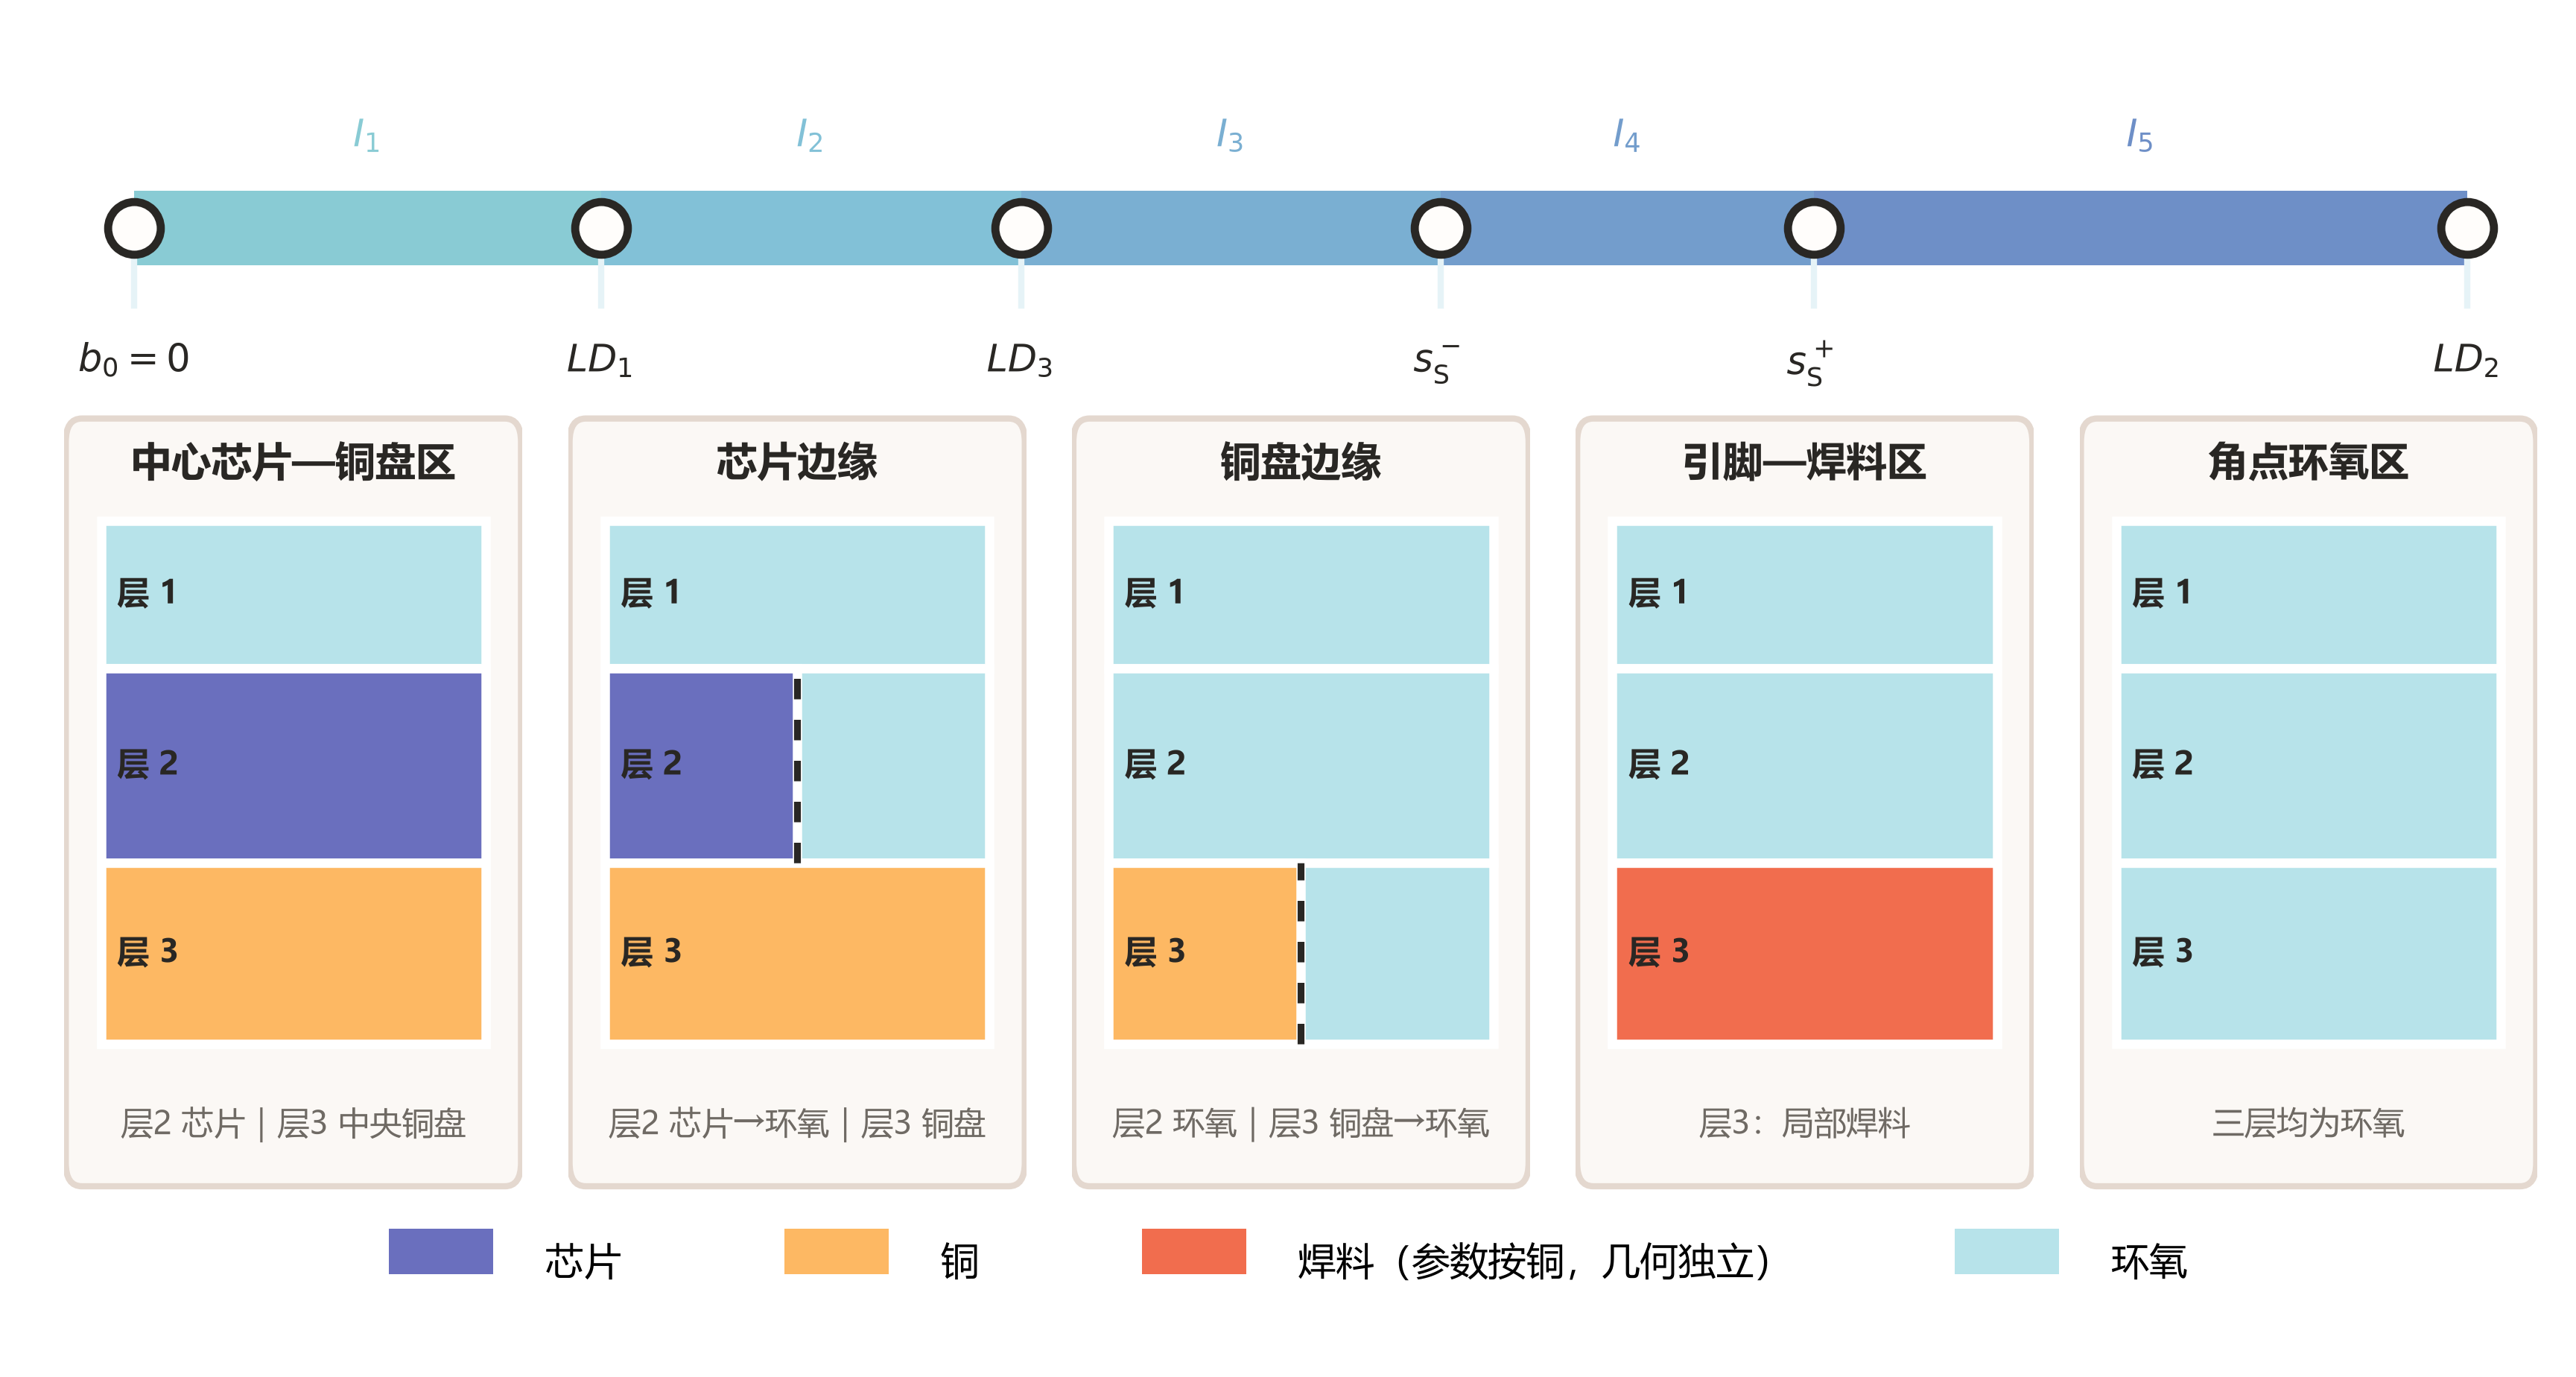
\includegraphics[width=1\textwidth]{output/figs/问题二QFN对角线路径分区示意.png}
  \caption{问题二：QFN对角线路径分区示意}\label{fig:q2-segments}
\end{figure}

图~\ref{fig:q2-segments}沿QFN中心至角点的半对角线将路径按几何占域划分为若干段，从左至右依次为：中心芯片—铜盘区、芯片边缘区、铜盘边缘区、引脚—焊料区、角点环氧区。各段因芯片、铜盘和焊料的存在与否而具有不同的层合结构，断点集合$\mathcal B$中的$b_0,LD_1,LD_3,s_S^-,s_S^+,LD_2$对应各段边界。

所有区段统一取参考线
\begin{equation}\label{eq:q2-zstar}
z_*=\frac{H_5}{2}.
\end{equation}
第$r$段的对角线应变为
\begin{equation}\label{eq:q2-strain}
\varepsilon_r(z)=\varepsilon_{0r}+(z-z_*)\kappa_r.
\end{equation}
利用式\eqref{eq:q2-Efield}和\eqref{eq:q2-Ealpha}在该段沿厚度积分，定义
\begin{equation}\label{eq:q2-ABDlocal}
A_r=\int_{z_0}^{z_3}E_r(z)\,\diff z,\quad
B_r=\int_{z_0}^{z_3}E_r(z)(z-z_*)\,\diff z,\quad
D_r=\int_{z_0}^{z_3}E_r(z)(z-z_*)^2\,\diff z,
\end{equation}
\begin{equation}\label{eq:q2-thermal}
n_r^T=\int_{z_0}^{z_3}E_r(z)\alpha_r(z)\,\diff z,\quad
m_r^T=\int_{z_0}^{z_3}E_r(z)\alpha_r(z)(z-z_*)\,\diff z.
\end{equation}
由于每段内部均为分片常材料，式\eqref{eq:q2-ABDlocal}和\eqref{eq:q2-thermal}可直接按各材料子域的上下界求和，无须再保留未使用的二维或有限宽积分公式。记
\begin{equation}\label{eq:q2-Kr}
\mathbf K_r=
\begin{bmatrix}A_r&B_r\\B_r&D_r\end{bmatrix},
\qquad
\mathbf t_r=
\begin{bmatrix}n_r^T\\m_r^T\end{bmatrix}.
\end{equation}
局部热弹性本构为
\begin{equation}\label{eq:q2-constitutive}
\begin{bmatrix}N\\M\end{bmatrix}
=\mathbf K_r
\begin{bmatrix}\varepsilon_{0r}\\\kappa_r\end{bmatrix}
-\mathbf t_r\Delta T.
\end{equation}

\begin{figure}[H]
  \centering
  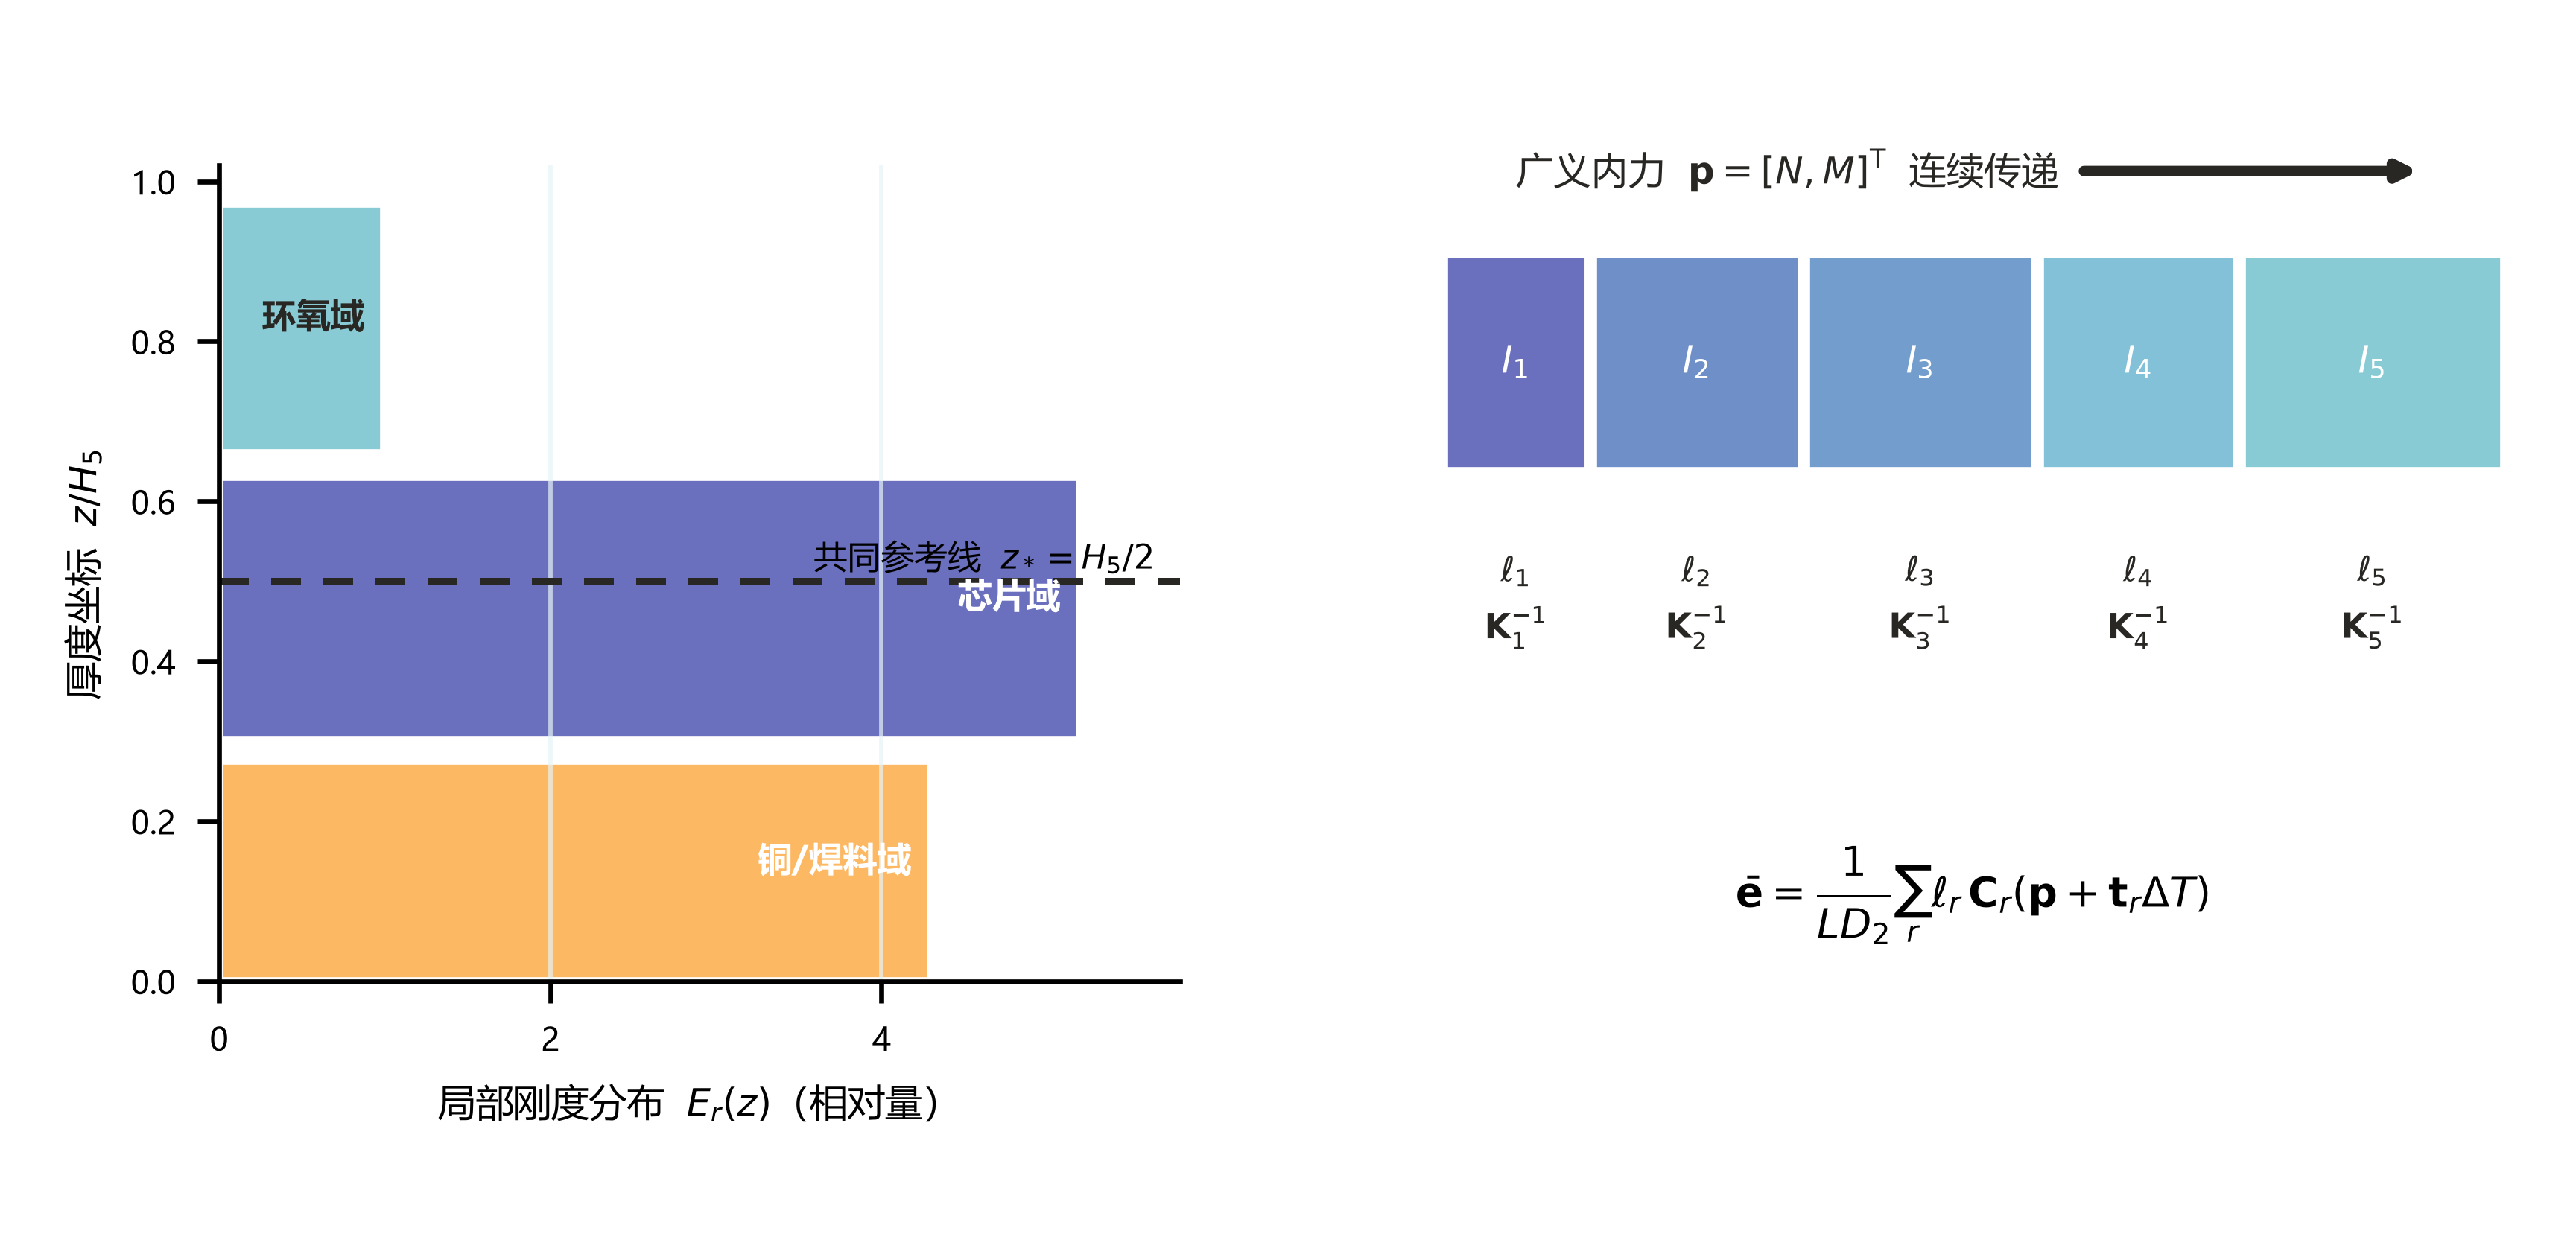
\includegraphics[width=1\textwidth]{output/figs/问题二QFN局部ABD到路径柔度串联.png}
  \caption{问题二：局部ABD截面到路径柔度串联示意}\label{fig:q2-abd-series}
\end{figure}

图~\ref{fig:q2-abd-series}左侧给出以$z_*=H_5/2$为共同参考线的局部截面材料分布，右侧示意广义内力$\mathbf p=[N,M]^{\mathsf T}$沿路径连续传递，各段以柔度矩阵$\mathbf K_r^{-1}$串联，整体平均应变由式~\eqref{eq:q2-Cbar}--\eqref{eq:q2-gbar}给出。

这里的$2\times2$ ABD是问题一变换截面模型的直接推广：$A_r$描述拉伸，$D_r$描述弯曲，$B_r$保留非对称截面产生的拉伸与弯曲耦合。

基础模型假设对角线窄条上无分布轴力和分布弯矩，因此广义内力$\mathbf p=[N,M]^{\mathsf T}$在各段连续，而各段应变和曲率可以不同。由式\eqref{eq:q2-constitutive}可得
\begin{equation}\label{eq:q2-localdef}
\begin{bmatrix}\varepsilon_{0r}\\\kappa_r\end{bmatrix}
=\mathbf K_r^{-1}(\mathbf p+\mathbf t_r\Delta T).
\end{equation}
各段沿长度是串联关系，应平均柔度而不是直接平均刚度：
\begin{equation}\label{eq:q2-Cbar}
\bar{\mathbf C}
=\frac{1}{LD_2}\sum_{r=1}^{R}\ell_r\mathbf K_r^{-1},
\end{equation}
\begin{equation}\label{eq:q2-gbar}
\bar{\mathbf g}
=\frac{1}{LD_2}\sum_{r=1}^{R}
\ell_r\mathbf K_r^{-1}\mathbf t_r.
\end{equation}
定义整体等效刚度与热载荷向量
\begin{equation}\label{eq:q2-Keq}
\mathbf K_{\mathrm{eq}}=\bar{\mathbf C}^{-1}
=\begin{bmatrix}
A_{\mathrm{eq}}&B_{\mathrm{eq}}\\
B_{\mathrm{eq}}&D_{\mathrm{eq}}
\end{bmatrix},
\end{equation}
\begin{equation}\label{eq:q2-teq}
\mathbf t_{\mathrm{eq}}
=\mathbf K_{\mathrm{eq}}\bar{\mathbf g}
=\begin{bmatrix}N_{\mathrm{eq}}^T\\M_{\mathrm{eq}}^T\end{bmatrix}.
\end{equation}
整体本构为
\begin{equation}\label{eq:q2-global}
\mathbf p
=\mathbf K_{\mathrm{eq}}\bar{\mathbf e}
-\mathbf t_{\mathrm{eq}}\Delta T.
\end{equation}

得到\textbf{等效ABD}后，我们先将参考线移至等效\textbf{弹性中性轴}。等效中性轴及关于中性轴的弯曲刚度为
\begin{equation}\label{eq:q2-neutral}
z_n=z_*+\frac{B_{\mathrm{eq}}}{A_{\mathrm{eq}}},
\qquad
D_n=D_{\mathrm{eq}}-\frac{B_{\mathrm{eq}}^2}{A_{\mathrm{eq}}}.
\end{equation}
等效热矩移至中性轴后为
\begin{equation}\label{eq:q2-MnTeq}
M_{n,\mathrm{eq}}^T
=M_{\mathrm{eq}}^T
-\frac{B_{\mathrm{eq}}}{A_{\mathrm{eq}}}N_{\mathrm{eq}}^T.
\end{equation}
在中性轴变量$\bar\varepsilon_n,\bar\kappa$下，整体本构化为
\begin{equation}\label{eq:q2-decoupled}
\begin{bmatrix}N\\M_n\end{bmatrix}
=
\begin{bmatrix}A_{\mathrm{eq}}&0\\0&D_n\end{bmatrix}
\begin{bmatrix}\bar\varepsilon_n\\\bar\kappa\end{bmatrix}
-
\begin{bmatrix}N_{\mathrm{eq}}^T\\M_{n,\mathrm{eq}}^T\end{bmatrix}
\Delta T.
\end{equation}

\subsection{求等效拉伸杨氏模量}

令$\bar\varepsilon_n=1,\bar\kappa=0,\Delta T=0$，由式\eqref{eq:q2-decoupled}有$N=A_{\mathrm{eq}}$。将该QFN窄条与厚度同为$H_5$的均质窄条在相同中性轴应变下等效，有$N=E_{\mathrm D,t}^{\mathrm{QFN}}H_5\bar\varepsilon_n$。代入$\bar\varepsilon_n=1$和$N=A_{\mathrm{eq}}$，得到
\begin{equation}\label{eq:q2-Edt}
E_{\mathrm D,t}^{\mathrm{QFN}}
=\frac{A_{\mathrm{eq}}}{H_5}.
\end{equation}
该工况规定拉力通过等效中性轴，延续问题一纯拉伸不附加弯矩的定义。

\subsection{求等效弯曲杨氏模量}

令$\bar\varepsilon_n=0,\bar\kappa=1,\Delta T=0$，由式\eqref{eq:q2-decoupled}有$M_n=D_n$。对同厚度均质窄条，关于中性轴的弯矩为$M_n=E_{\mathrm D,b}^{\mathrm{QFN}}(H_5^3/12)\bar\kappa$。代入$\bar\kappa=1$和$M_n=D_n$，得到
\begin{equation}\label{eq:q2-Edb}
E_{\mathrm D,b}^{\mathrm{QFN}}
=\frac{12D_n}{H_5^3}
=\frac{12}{H_5^3}
\left(D_{\mathrm{eq}}-
\frac{B_{\mathrm{eq}}^2}{A_{\mathrm{eq}}}\right).
\end{equation}

\subsection{求等效热膨胀系数}

令$\Delta T=1,N=0,M_n=0$，由式\eqref{eq:q2-decoupled}的轴力方程可得中性轴处自由热应变与温升之比：
\begin{equation}\label{eq:q2-alpha}
\alpha_{\mathrm D}^{\mathrm{QFN}}
=\bar\varepsilon_n
=\frac{N_{\mathrm{eq}}^T}{A_{\mathrm{eq}}},
\end{equation}
并可同时得到辅助量
\begin{equation}\label{eq:q2-kappaT}
\kappa_T
=\bar\kappa
=\frac{M_{n,\mathrm{eq}}^T}{D_n}.
\end{equation}
式\eqref{eq:q2-Edt}至\eqref{eq:q2-alpha}给出题目要求的三个等效参数；式\eqref{eq:q2-kappaT}表征非对称QFN在自由热膨胀下的翘曲曲率，作为辅助输出量。

为将三个等效参数整理为紧凑的形式，记
\begin{equation}\label{eq:q2-kmatrix}
\mathbf K_{\mathrm{eq}}
=\bar{\mathbf C}^{-1}
=\begin{bmatrix}k_{11}&k_{12}\\k_{12}&k_{22}\end{bmatrix},
\qquad
\mathbf t_{\mathrm{eq}}=\mathbf K_{\mathrm{eq}}\bar{\mathbf g}
=\begin{bmatrix}N_{\mathrm{eq}}^T\\M_{\mathrm{eq}}^T\end{bmatrix}.
\end{equation}
其中$\bar{\mathbf C}$和$\bar{\mathbf g}$已由每段题图几何、材料参数通过式\eqref{eq:q2-ABDlocal}至\eqref{eq:q2-gbar}唯一确定。由此得到三个等效参数的显式符号表达式
\begin{equation}\label{eq:q2-final}
E_{\mathrm D,t}^{\mathrm{QFN}}=\frac{k_{11}}{H_5},\qquad
E_{\mathrm D,b}^{\mathrm{QFN}}
=\frac{12}{H_5^3}\left(k_{22}-\frac{k_{12}^2}{k_{11}}\right),\qquad
\alpha_{\mathrm D}^{\mathrm{QFN}}=\frac{N_{\mathrm{eq}}^T}{k_{11}}.
\end{equation}


我们对模型进行如下解析退化与自洽性检查。当$LD_1\to0$时芯片占域消失，第二层相应区域退化为环氧；当$LD_1\to LD_2$时芯片沿整条对角线路径铺满第二层。两种极限均由\textbf{断点集合}与指示函数自动实现，无需修改主公式。当$LD_3\to0$时中央铜盘贡献消失；当$LD_3\to LD_2$时铜盘沿整条路径铺满第三层的相应厚度区域。当$s_{\mathrm S}^+-s_{\mathrm S}^-\to0$或$H_1\to0$时，焊料贡献应连续消失。当焊料域铺满第三层中由题图指定的可占区域时，$\chi_{\mathrm S}$应趋于该区域的指示函数；由于$E_{\mathrm{sol}}=E_{\mathrm c},\alpha_{\mathrm{sol}}=\alpha_{\mathrm c}$，该区域应等价为完整铜参数区。若全部材料具有相同$E,\alpha$，则可得$E_{\mathrm D,t}^{\mathrm{QFN}}=E_{\mathrm D,b}^{\mathrm{QFN}}=E,\alpha_{\mathrm D}^{\mathrm{QFN}}=\alpha,\kappa_T=0$。若所有区段的$\mathbf K_r,\mathbf t_r$完全相同，则$\bar{\mathbf C}=\mathbf K_r^{-1},\mathbf K_{\mathrm{eq}}=\mathbf K_r,\mathbf t_{\mathrm{eq}}=\mathbf t_r$，此时式\eqref{eq:q2-Edt}至\eqref{eq:q2-alpha}分别退化为问题一的$E_{d,t}=S_0/h,E_{d,b}=12J/h^3,\alpha_d=T_0/S_0$，构成问题一至问题二最直接的承接验证。每段满足$A_r>0,D_r>0,A_rD_r-B_r^2>0$，且$A$的量纲为N/m、$B$为N、$D$为N$\cdot$m，两个模量为Pa，热膨胀系数为K$^{-1}$。

我们按以下步骤完成问题二的计算，如算法\ref{alg:q2}所示。

\begin{algorithm}[H]
\caption{问题二等效参数计算流程}\label{alg:q2}
\begin{algorithmic}[1]
\Require 题图给出的QFN各层几何与材料参数
\Ensure $E_{\mathrm D,t}^{\mathrm{QFN}},E_{\mathrm D,b}^{\mathrm{QFN}},\alpha_{\mathrm D}^{\mathrm{QFN}}$
\State 确定三层界面、芯片域、铜盘域与焊料域，按题图读取界面坐标并取$H_5=z_3-z_0$，统一取$z_0=0$、$z_*=H_5/2$；仅当题图确认焊料位于QFN本体总厚度内时$H_1$才计入$H_5$，否则$H_1$仅用于定位第三层内焊料子域，不进入总厚度
\State 构造断点集合$\mathcal B=\{0,LD_1,LD_3,s_{\mathrm S}^-,s_{\mathrm S}^+,LD_2\}$，$\ell_r=b_r-b_{r-1}>0$，确定各区段材料组成
\State 计算每段局部刚度与热载荷：
\[
A_r=\int_{z_0}^{z_3}E_r(z)\,\diff z,\;
B_r=\int_{z_0}^{z_3}E_r(z)(z-z_*)\,\diff z,\;
D_r=\int_{z_0}^{z_3}E_r(z)(z-z_*)^2\,\diff z.
\]
\State 路径柔度串联，得到等效ABD与等效热载荷：
\[
\bar{\mathbf C}=\frac{1}{LD_2}\sum_{r=1}^{R}\ell_r\mathbf K_r^{-1},\qquad
\mathbf K_{\mathrm{eq}}=\bar{\mathbf C}^{-1}
=\begin{bmatrix}A_{\mathrm{eq}}&B_{\mathrm{eq}}\\B_{\mathrm{eq}}&D_{\mathrm{eq}}\end{bmatrix}.
\]
\State 移至等效中性轴并输出三个等效参数：
\[
z_n=z_*+\frac{B_{\mathrm{eq}}}{A_{\mathrm{eq}}},\qquad
D_n=D_{\mathrm{eq}}-\frac{B_{\mathrm{eq}}^2}{A_{\mathrm{eq}}},\qquad
E_{\mathrm D,t}^{\mathrm{QFN}}=\frac{A_{\mathrm{eq}}}{H_5},\;
E_{\mathrm D,b}^{\mathrm{QFN}}=\frac{12D_n}{H_5^3},\;
\alpha_{\mathrm D}^{\mathrm{QFN}}=\frac{N_{\mathrm{eq}}^T}{A_{\mathrm{eq}}}.
\]
\State 执行消失、铺满、均质、无分段、正定性和量纲检查，要求$A_r>0$，$D_r>0$，$A_rD_r-B_r^2>0$，$[E]=\mathrm{Pa}$，$[\alpha]=\mathrm{K}^{-1}$
\State \Return $E_{\mathrm D,t}^{\mathrm{QFN}},E_{\mathrm D,b}^{\mathrm{QFN}},\alpha_{\mathrm D}^{\mathrm{QFN}}$
\end{algorithmic}
\end{algorithm}


%================ 6 问题三 =================

\section{问题三：实际BGA封装角点的\textbf{等效热弹性参数}估计}

问题一将焊球阵列均匀化为连续连接层，能够快速估计BGA与PCB组合结构的整体热弹性参数，但没有保留实际阵列中的中心空隙、外环结构和角点缺球。题目给出的实际阵列由$23\times23$外部格点、$13\times13$中部空区和$9\times9$中心阵列构成，且四个最外角位置没有焊球，焊球总数为437。封装角点距离中性点最远，外角焊球缺失虽然只改变少量连接点，却可能显著改变角点位移和邻近焊球载荷，因此我们需要在模型中显式保留缺球的位置信息。在方法选择上，全局均匀化能够直接计算整体等效参数，却不能识别缺球位置；二维离散模型能够保留实际拓扑，但主要输出位移、载荷和能量等响应量。基于这一分工，我们以\textbf{角点窗口修正的分段ABD模型}作为估计整体参数的主模型，以\textbf{二维壳-离散弹簧模型}作为校核局部响应的验证模型。我们的初步思路是：沿封装中心至角点的对角线建立单位宽度层合窄条，用\textbf{等效柔度截面积}修正单个焊球刚度；按局部结构差异将路径划分为芯片覆盖段、中段和\textbf{角点窗口段}三段，角点窗口段内的连接层模量按窗口内实际焊球计数局部折算，使角点缺球直接进入主模型；随后由分段ABD柔度串联得到\textbf{等效拉伸杨氏模量}、\textbf{等效弯曲杨氏模量}和\textbf{等效热膨胀系数}；最后用二维面内壳和离散剪切弹簧分别计算437、441两种阵列的整体能量、角点相对位移和最近角点焊球载荷，检验均匀化模型对整体量和局部量的适用范围。其中，截面线性应变分布及拉伸、耦合、弯曲刚度的构造遵循经典层合板理论$^{\textbf{[\ref{ref:3}]}}$。



从继承关系看，问题三复用了问题一离散焊球折算为等效连接层的均匀化思想，问题二路径分段加柔度串联的框架；与问题二不同的是，分段依据不再是材料层边界，而是\textbf{实际焊球拓扑导致的连接状态边界}。问题一没有焊球几何细节，只能采用面积占比$\phi$折算；问题三给出焊球直径、高度和焊盘尺寸，因此升级为等效柔度截面积与单球剪切刚度标定，二者分别服务于“轴向拉伸与弯曲的几何面积均匀化”和“层间剪切传力的局部连接器标定”两种工况。


问题三涉及的主要符号如下表所示。

\begin{table}[H]\centering
  \caption{问题三主要符号说明}\label{tab:symbol-q3}
  \small
  \begin{tabular}{ccc}
    \toprule
    符号 & 说明 & 单位 \\
    \midrule
    $L$ & BGA封装边长 & m \\
    $p$ & 相邻焊球球心间距 & m \\
    $s,n$ & 对角线方向和横向坐标 & m \\
    $h$ & BGA-焊球-PCB等效截面总厚度 & m \\
    $h_{\mathrm b}$ & 桶形焊料本体高度 & m \\
    $r_{\mathrm p},r_{\mathrm m}$ & 焊球端部半径、最大半径 & m \\
    $A_{\mathrm{bar}}$ & 桶体等柔度面积 & m$^2$ \\
    $A_{G,\mathrm{eq}}$ & 含上下焊盘的单连接器等柔度面积 & m$^2$ \\
    $k_G$ & 单个焊球连接器的面内剪切刚度 & N/m \\
    $w$ & 角点窗口沿对角线的长度 & m \\
    $N_{\mathrm c}$ & 窗口内实际焊球数 & 无量纲 \\
    $E_{\mathrm c}$ & 全局折算连接层模量 & Pa \\
    $E_{\mathrm c}^{\mathrm{win}}$ & 窗口段连接层局部折算模量 & Pa \\
    $d_{\min}$ & 最近焊球到角点的距离 & m \\
    $\mathbf K_r,\mathbf t_r$ & 第$r$段标量ABD刚度矩阵、热载荷向量 & 混合量纲 \\
    $A_{\mathrm{eq}},B_{\mathrm{eq}},D_{\mathrm{eq}}$ & 路径等效拉伸、耦合和弯曲刚度 & N/m, N, N$\cdot$m \\
    $z_{\mathrm n}$ & 等效弹性中性轴距PCB底面的坐标 & m \\
    $D_{\mathrm n}$ & 关于等效中性轴的弯曲刚度 & N$\cdot$m \\
    $E_{\mathrm{d,t}},E_{\mathrm{d,b}},\alpha_{\mathrm d}$ & 沿对角线方向的三个等效参数 & Pa, Pa, 1/K \\
    \bottomrule
  \end{tabular}
\end{table}

下标$\mathrm{PCB},\mathrm{sub},\mathrm m,\mathrm{die},\mathrm s,\mathrm p$分别表示PCB、基板、覆膜、芯片、焊料和焊盘。

由于题目关注角点沿对角线方向的热弹性响应，我们将平面坐标投影到对角线与横向构成的正交坐标系，以统一描述焊球位置和中心至角点的传力路径。以BGA中心为原点，取右上角方向为正方向，对角线和横向单位向量分别定义为
\begin{equation}\label{eq:q3-ed}
\mathbf e_{\mathrm d}=\frac{1}{\sqrt 2}(1,1)^{\mathsf T},\qquad
\mathbf e_{\mathrm n}=\frac{1}{\sqrt 2}(1,-1)^{\mathsf T},
\end{equation}
平面内位置向量$\mathbf x=(x,y)^{\mathsf T}$的路径坐标和横向坐标为
\begin{equation}\label{eq:q3-sn}
s=\mathbf e_{\mathrm d}^{\mathsf T}\mathbf x,\qquad
n=\mathbf e_{\mathrm n}^{\mathsf T}\mathbf x.
\end{equation}
中心到角点的路径长度为$L_{\mathrm D}=L/\sqrt 2$。

由题图推断，焊球排布存在同心方框状区域焊球缺失和角部顶点缺失的情况。设4个顶点焊球均缺失，球阵宽n，缺失区外宽m，内宽p，因此有$n^2-m^2+p^2-4=437$。
枚举可能解，得到满足要求且几何分布最合理的排列方式：\textbf{n=23，m=13，p=9}

将二维焊球阵列降为对角线窄条会改变单元代表面积，因此我们按面积守恒确定条带宽度，避免降维过程人为改变连接层的计算尺度。真实焊球网格单元面积为$p^2$，正方形网格沿对角线的穿越长度为$\ell_{\mathrm d}=\sqrt2\,p$。令\textbf{等面积条带宽度}$b_{\mathrm{eq}}$满足
\begin{equation}\label{eq:q3-beq}
b_{\mathrm{eq}}\ell_{\mathrm d}=p^2
\quad\Longrightarrow\quad
b_{\mathrm{eq}}=\frac{p}{\sqrt2}.
\end{equation}
基准节距$p=1.0$ mm时，$b_{\mathrm{eq}}=0.707107$ mm。若直接令条带宽度等于$p$，每个对角线单元的面积将被放大为$\sqrt2\,p^2$，连接层折算刚度随之被高估。

已有研究通常将BGA焊点视为由母线旋转形成的轴对称曲面，并利用焊料体积、焊盘半径和表面张力等条件预测焊点外形$^{\textbf{[\ref{ref:9}]}}$。题目只给出焊球端部直径和最大直径，
无法唯一恢复真实母线，因此我们采用满足已知尺寸和几何对称性的抛物线重构桶形轮廓。焊球连接体总高为$H=0.50$ mm，上下焊盘高度分别为$h_{\mathrm l}=0.03$ mm、$h_{\mathrm u}=0.02$ mm，因此桶形焊料本体高度为
$
h_{\mathrm b}=H-h_{\mathrm l}-h_{\mathrm u}=0.45\ \mathrm{mm}.
$
取焊球端部半径$r_{\mathrm p}=0.25$ mm、中部最大半径$r_{\mathrm m}=0.35$ mm，在$0\le z\le h_{\mathrm b}$上构造母线与截面积
\begin{equation}\label{eq:q3-rz}
r(z)=r_{\mathrm p}+
4(r_{\mathrm m}-r_{\mathrm p})\frac{z}{h_{\mathrm b}}
\left(1-\frac{z}{h_{\mathrm b}}\right),
\qquad
A(z)=\pi r^2(z).
\end{equation}
桶形焊球各高度处截面积不同，且各截面薄片在剪切传力方向上串联，因此我们按柔度积分定义等效面积，而不采用截面积的算术平均：
\begin{equation}\label{eq:q3-abar}
A_{\mathrm{bar}}
=\frac{h_{\mathrm b}}
{\displaystyle\int_0^{h_{\mathrm b}}\frac{1}{A(z)}\,\diff z}.
\end{equation}
焊料本体与上下焊盘沿同一传力路径依次变形，三者的柔度直接相加，由此得到单个完整连接器的剪切刚度。令$G_{\mathrm s}=E_{\mathrm s}/[2(1+\nu_{\mathrm s})]$、$G_{\mathrm p}=E_{\mathrm p}/[2(1+\nu_{\mathrm p})]$，单个连接器的剪切柔度和剪切刚度为
\begin{equation}\label{eq:q3-cg}
C_G=\frac{h_{\mathrm l}}{G_{\mathrm p}A_{\mathrm l}}
+\int_0^{h_{\mathrm b}}\frac{1}{G_{\mathrm s}A(z)}\,\diff z
+\frac{h_{\mathrm u}}{G_{\mathrm p}A_{\mathrm u}},
\qquad
k_G=C_G^{-1},
\end{equation}
式中$A_{\mathrm l}$和$A_{\mathrm u}$分别为上下焊盘面积。需要说明这里的接口假设：单球剪切刚度$k_G$描述的是PCB与BGA相对面内位移的阻抗，属于面向层间剪切传力的局部连接器标定；为进入标量ABD框架，我们将离散连接器等效为具有相同平均剪切柔度的连续连接层，并令该层在截面内与其他层共享轴向应变和曲率。因此式\eqref{eq:q3-ageq}得到的剪切等效面积先代入全局剪切刚度等价关系得到$G_{\mathrm c}$，再转换为标量ABD中的接口模量$E_{\mathrm c}$；该转换是让剪切标定结果进入一维拉伸—弯曲框架的近似映射，并非问题一面积占比$\phi E_2$的简单替换，其代价正是后文由二维壳-离散弹簧模型校核的共同响应假设。为与标量ABD模型连接，我们将上式转换为总高$H$上的单连接器等柔度面积：
\begin{equation}\label{eq:q3-ageq}
A_{G,\mathrm{eq}}=\frac{H}{G_{\mathrm s}C_G}.
\end{equation}
数值积分得到
$
A_{\mathrm{bar}}=0.305935\ \mathrm{mm^2},
A_{G,\mathrm{eq}}=0.315299\ \mathrm{mm^2},
k_G=11.67775\ \mathrm{MN/m}.
$
作为对比，简单焊盘面积为$\pi(0.25)^2=0.196350\ \mathrm{mm^2}$，桶体等柔度面积为其1.558倍，说明将焊球直接替换成焊盘等截面圆柱会明显低估单球刚度。

为使离散焊球能够进入连续层合截面计算，我们依据总体剪切刚度等价原则，将全部焊球折算为具有相同平均连接能力的连续连接层。设BGA平面面积为$L^2$，共有$N$个有效焊球，令连续连接层与全部离散连接器具有相同的平均剪切柔度，可得全局折算剪切模量和标量ABD接口模量：
\begin{equation}\label{eq:q3-ec}
G_{\mathrm c}=\frac{Nk_GH}{L^2},\qquad
E_{\mathrm c}=2(1+\nu_{\mathrm s})G_{\mathrm c}.
\end{equation}
代入两种阵列的球数，得到
$
E_{\mathrm c}^{(437)}=10.19126\ \mathrm{GPa},
E_{\mathrm c}^{(441)}=10.28454\ \mathrm{GPa}.
$
连接层热膨胀系数按自由串联伸长等效：
\begin{equation}\label{eq:q3-alphac}
\alpha_{\mathrm c}
=\frac{\alpha_{\mathrm s}h_{\mathrm b}
+\alpha_{\mathrm p}(h_{\mathrm l}+h_{\mathrm u})}{H}
=21.5\ \mathrm{ppm/K}.
\end{equation}
式\eqref{eq:q3-ec}对应全局平均密度下的折算，对角线路径中段和芯片段仍使用该全局值，角点窗口段改用下文的窗口局部折算值。该式不描述空隙区的局部绕行传力，空隙两侧焊球的横向桥接由二维离散连接模型保留。

下面建立\textbf{三区段ABD柔度等效模型}。组合截面总厚度为
$
h=h_{\mathrm{PCB}}+H+h_{\mathrm{sub}}+h_{\mathrm m}=4.07\ \mathrm{mm},
$
中央芯片在对角线路径上的终点为
$
s_{\mathrm{die}}=\frac{L_{\mathrm{die}}}{\sqrt2}=3.18198\ \mathrm{mm}.
$
全局折算模量会抹去四个外角缺球的位置差异，因此我们在角点附近设置与对角线路径对齐的局部窗口，使缺球拓扑能够进入主模型。取窗口为角点处的等腰直角三角形区域
\begin{equation}\label{eq:q3-window}
\Omega_w=\left\{\mathbf x\in[-L/2,L/2]^2\ \middle|\ s(\mathbf x)\ge L_{\mathrm D}-w\right\},
\qquad
A(\Omega_w)=w^2,
\end{equation}
其斜边长为$w\sqrt2$，面积恰为$w^2$，基准取$w=3p=3$ mm。该选择与路径坐标$s$天然对齐：窗口在路径上的投影恰为区间$(L_{\mathrm D}-w,L_{\mathrm D}]$，无需额外的几何近似即可作为第三区段。窗口内焊球计数为
\begin{equation}\label{eq:q3-nc}
N_{\mathrm c}=\#\left\{(i,j)\in\mathcal S:\ \frac{(i+j)p}{\sqrt2}\ge L_{\mathrm D}-w\right\}.
\end{equation}
对右上角点，437阵列的最近焊球为$(10,11)$和$(11,10)$，其对角线坐标$s=21p/\sqrt2\approx14.849$ mm，距角点$3.536$ mm，大于$3p$，故窗口内无球，$N_{\mathrm c}=0$；441阵列的外角球$(11,11)$落在窗口内，$N_{\mathrm c}=1$。为保持局部模型与全局模型采用相同的单球刚度口径，我们以窗口内实际球数与窗口面积之比折算局部连接层模量：
\begin{equation}\label{eq:q3-ecwin}
E_{\mathrm c}^{\mathrm{win}}
=2(1+\nu_{\mathrm s})\,\frac{N_{\mathrm c}k_GH}{w^2}.
\end{equation}
式\eqref{eq:q3-ecwin}与式\eqref{eq:q3-ec}的唯一差别是把全局球数与全局面积换成窗口球数与窗口面积，因此当窗口密度恰好等于全局平均密度时$E_{\mathrm c}^{\mathrm{win}}=E_{\mathrm c}$，三区段模型严格退化为两区段模型，这是该改造的内在一致性条件，不引入新假设。若$N_{\mathrm c}=0$，窗口段连接层缺席，其刚度与热载荷取零，PCB、基板、覆膜等连续层照常承载。基准$w=3p$下，
$
E_{\mathrm c}^{\mathrm{win}}(437)=0,
E_{\mathrm c}^{\mathrm{win}}(441)=1.75166\ \mathrm{GPa},
$
两者均显著低于全局值$10.19\sim10.28$ GPa，表明角部3 mm范围是连接刚度的低谷区，这正是全局均匀化所抹去的信息。

于是路径分为三段：区段$I_1=[0,s_{\mathrm{die}}]$包含PCB、连接层（全局$E_{\mathrm c}$）、基板、芯片和芯片上覆膜；区段$I_2=(s_{\mathrm{die}},L_{\mathrm D}-w]$包含PCB、连接层（全局$E_{\mathrm c}$）、基板和完整覆膜；区段$I_3=(L_{\mathrm D}-w,L_{\mathrm D}]$包含PCB、连接层（窗口$E_{\mathrm c}^{\mathrm{win}}$）、基板和完整覆膜。

\begin{figure}[H]
  \centering
  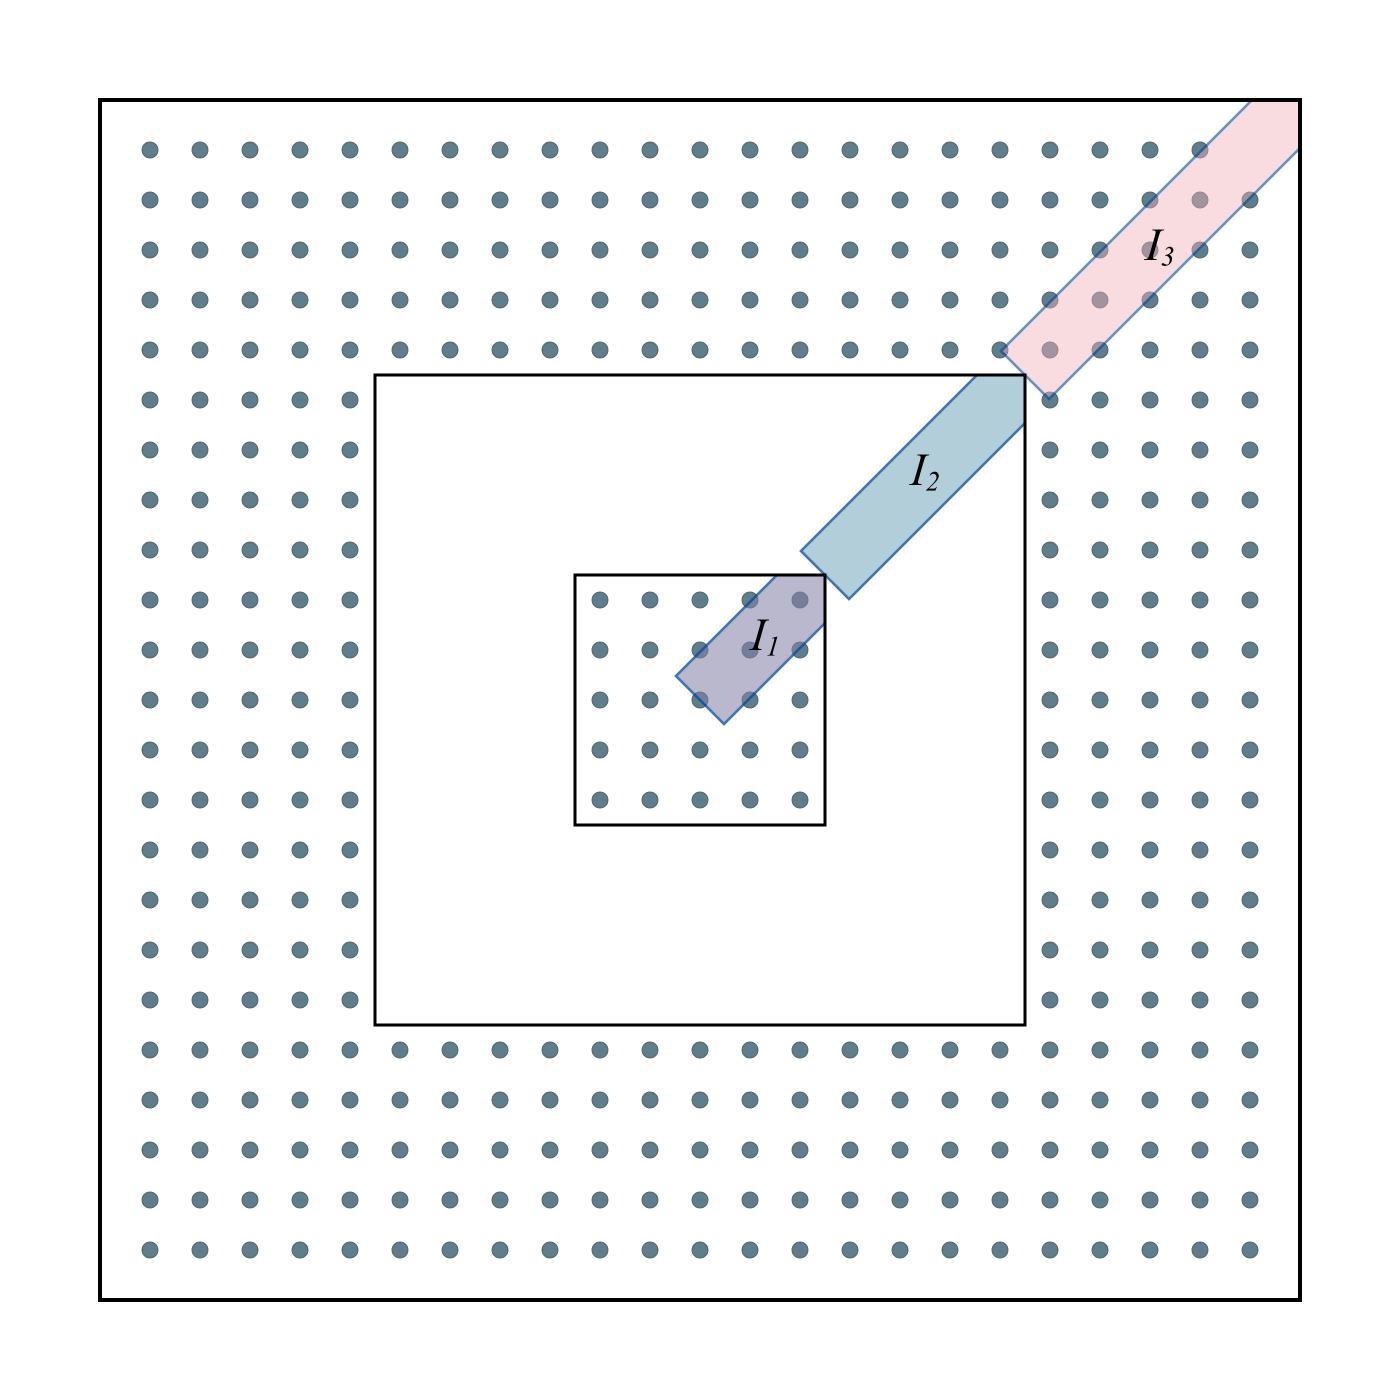
\includegraphics[width=0.6\textwidth]{output/figs/问题三BGA_对角线三区段.png}
  \caption{问题三：BGA对角线三区段划分}\label{fig:q3-segments}
\end{figure}

图~\ref{fig:q3-segments}给出BGA封装对角线方向的三区段几何示意：$I_1$为芯片覆盖段，$I_2$为芯片外缘至角点窗口前缘的中段，角点窗口$I_3$为距角点$w=3p$的等腰直角三角形区域。三段的连接层模量分别采用全局折算值$E_{\mathrm c}$与窗口局部值$E_{\mathrm c}^{\mathrm{win}}$。

BGA各材料层沿厚度方向非对称分布，层间热失配会同时引起面内伸长与弯曲，因此我们采用ABD理论统一描述轴向应变、曲率及二者的耦合。在\textbf{拉伸弯曲共同响应假设}下，代理连接层与相邻PCB、基板共享截面轴向应变和曲率，不能只作为面内拉伸层计入$A_r$，而应与其他连续层一样按其厚度坐标同时贡献$A_r$、$B_r$和$D_r$。统一以PCB底面为$z=0$，取参考面$z_*=h/2$，第$r$段沿对角线的应变场为
\begin{equation}\label{eq:q3-strain}
\varepsilon_r(z)=\varepsilon_{0r}+(z-z_*)\kappa_r.
\end{equation}
根据线弹性热应力关系，对第$r$段沿厚度积分，得到局部ABD刚度和热载荷：
\begin{equation}\label{eq:q3-abd}
A_r=\int_0^h E_r(z)\,\diff z,\quad
B_r=\int_0^h E_r(z)(z-z_*)\,\diff z,\quad
D_r=\int_0^h E_r(z)(z-z_*)^2\,\diff z,
\end{equation}
\begin{equation}\label{eq:q3-thermal}
n_r^{\mathrm{th}}=\int_0^h E_r(z)\alpha_r(z)\,\diff z,\quad
m_r^{\mathrm{th}}=\int_0^h E_r(z)\alpha_r(z)(z-z_*)\,\diff z.
\end{equation}
记
\begin{equation}\label{eq:q3-kr}
\mathbf K_r=
\begin{bmatrix}A_r&B_r\\B_r&D_r\end{bmatrix},
\qquad
\mathbf t_r=
\begin{bmatrix}n_r^{\mathrm{th}}\\m_r^{\mathrm{th}}\end{bmatrix},
\end{equation}
则第$r$段的热弹性本构关系为
\begin{equation}\label{eq:q3-constitutive}
\begin{bmatrix}N\\M\end{bmatrix}
=\mathbf K_r
\begin{bmatrix}\varepsilon_{0r}\\\kappa_r\end{bmatrix}
-\mathbf t_r\Delta T.
\end{equation}

\begin{figure}[H]
  \centering
  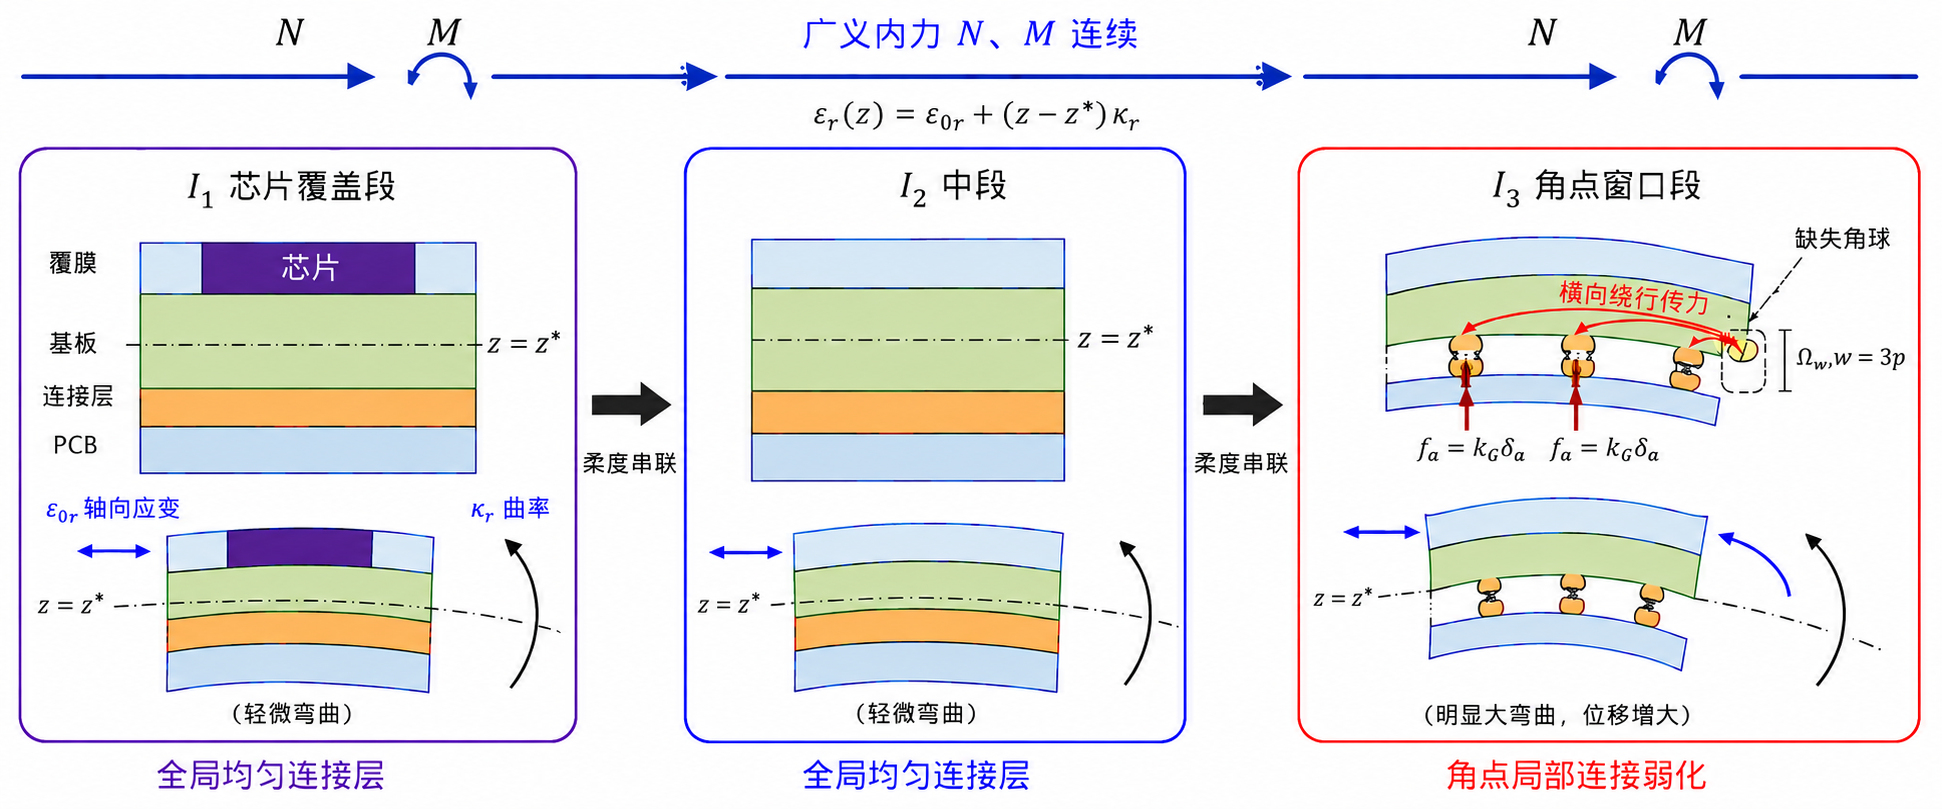
\includegraphics[width=0.95\textwidth]{output/figs/问题三_三区段传力与应变曲率示意图.png}
  \caption{问题三：三区段传力与应变曲率示意}\label{fig:q3-strain-curvature}
\end{figure}

图~\ref{fig:q3-strain-curvature}对比了$I_1$芯片覆盖段与$I_2$中段的截面结构差异：$I_1$段在基板上方存在芯片层，$I_2$段则无芯片；两段均包含覆膜、基板、连接层和PCB。广义内力$N,M$沿路径连续传递，各层共享轴向应变$\varepsilon_{0r}$和曲率$\kappa_r$，截面呈线性应变分布，如式~\eqref{eq:q3-strain}所示。

三个路径区段串联传递相同的广义内力$N,M$，但产生不同的应变和曲率，因此路径等效时我们对柔度作长度加权，而不直接平均刚度：
\begin{equation}\label{eq:q3-cbar}
\bar{\mathbf C}
=\frac{1}{L_{\mathrm D}}\sum_{r=1}^{3}\ell_r\mathbf K_r^{-1},
\qquad
\bar{\mathbf g}
=\frac{1}{L_{\mathrm D}}\sum_{r=1}^{3}
\ell_r\mathbf K_r^{-1}\mathbf t_r,
\end{equation}
式中$\ell_1=s_{\mathrm{die}}$，$\ell_2=L_{\mathrm D}-w-s_{\mathrm{die}}$，$\ell_3=w$。路径等效刚度与单位温升热载荷为
\begin{equation}\label{eq:q3-keq}
\mathbf K_{\mathrm{eq}}
=\bar{\mathbf C}^{-1}
=\begin{bmatrix}
A_{\mathrm{eq}}&B_{\mathrm{eq}}\\
B_{\mathrm{eq}}&D_{\mathrm{eq}}
\end{bmatrix},
\qquad
\mathbf t_{\mathrm{eq}}
=\mathbf K_{\mathrm{eq}}\bar{\mathbf g}
=\begin{bmatrix}
N_{\mathrm{eq}}^{\mathrm{th}}\\M_{\mathrm{eq}}^{\mathrm{th}}
\end{bmatrix}.
\end{equation}
将参考面移动到等效弹性中性轴，得到
\begin{equation}\label{eq:q3-neutral}
z_{\mathrm n}=z_*+\frac{B_{\mathrm{eq}}}{A_{\mathrm{eq}}},
\qquad
D_{\mathrm n}=D_{\mathrm{eq}}-
\frac{B_{\mathrm{eq}}^2}{A_{\mathrm{eq}}}.
\end{equation}
我们分别定义拉伸、弯曲和自由热膨胀工况，以避免用单一杨氏模量混合表征不同受载机制，使三个等效参数的物理含义保持清晰。最终三个等效参数为
\begin{equation}\label{eq:q3-final}
E_{\mathrm{d,t}}=\frac{A_{\mathrm{eq}}}{h},\qquad
E_{\mathrm{d,b}}=\frac{12D_{\mathrm n}}{h^3},\qquad
\alpha_{\mathrm d}=\frac{N_{\mathrm{eq}}^{\mathrm{th}}}{A_{\mathrm{eq}}}.
\end{equation}
式中，$E_{\mathrm{d,t}}$由单位中性轴拉伸工况定义，$E_{\mathrm{d,b}}$由单位纯弯曲工况定义，$\alpha_{\mathrm d}$为无轴力、无中性轴弯矩时的自由热应变系数，三个输出对应不同的定义工况。需要指出，三段划分并未改变串联公式的形式：式\eqref{eq:q3-cbar}相对原两区段模型仅把求和上限从2改为3，角点窗口正是以第三区段的身份复用原有框架，而非附加的经验修正。

求解时，桶形截面积随高度非线性变化，相应柔度积分不便直接解析计算，因此我们采用96点Gauss-Legendre求积完成数值求解。对任意函数$f(z)$，
\begin{equation}\label{eq:q3-gauss}
\int_0^{h_{\mathrm b}}f(z)\,\diff z
\approx\frac{h_{\mathrm b}}{2}
\sum_{q=1}^{96}w_q
f\!\left[\frac{h_{\mathrm b}}{2}(1+\xi_q)\right],
\end{equation}
式中$\xi_q$和$w_q$分别为标准区间$[-1,1]$上的求积节点和权重。将上式代入式\eqref{eq:q3-abar}至\eqref{eq:q3-ecwin}，再由式\eqref{eq:q3-abd}至\eqref{eq:q3-final}完成矩阵计算。基准窗口$w=3p$下，437阵列的主要中间量如表\ref{tab:q3-mid}所示。

\begin{table}[H]\centering
  \caption{437阵列主要中间量（$w=3p$）}\label{tab:q3-mid}
  \small
  \begin{tabular}{ccc}
    \toprule
    \textbf{中间量} & \textbf{数值} & \textbf{单位} \\
    \midrule
    $A_{\mathrm{eq}}$ & $1.253613\times10^8$ & N/m \\
    $B_{\mathrm{eq}}$ & $-7.228340\times10^3$ & N \\
    $D_{\mathrm{eq}}$ & $1.288212\times10^2$ & N$\cdot$m \\
    $D_{\mathrm n}$ & $1.284044\times10^2$ & N$\cdot$m \\
    $N_{\mathrm{eq}}^{\mathrm{th}}$ & $2.416607\times10^3$ & N/(m$\cdot$K) \\
    $z_{\mathrm n}$ & 1.977340 & mm \\
    \bottomrule
  \end{tabular}
\end{table}

由式\eqref{eq:q3-final}得到437阵列的主结果为$E_{\mathrm{d,t}}=30.80129$ GPa、$E_{\mathrm{d,b}}=22.85483$ GPa和$\alpha_{\mathrm d}=19.27714$ ppm/K，441阵列的相应结果为$E_{\mathrm{d,t}}=30.84987$ GPa、$E_{\mathrm{d,b}}=22.85597$ GPa和$\alpha_{\mathrm d}=19.28007$ ppm/K。

我们按以下步骤完成问题三的计算，如算法\ref{alg:q3}所示。

\begin{algorithm}[H]
\caption{问题三等效参数计算流程}\label{alg:q3}
\begin{algorithmic}[1]
\Require 题给BGA几何、材料参数及焊球拓扑
\Ensure $E_{\mathrm{d,t}},E_{\mathrm{d,b}},\alpha_{\mathrm d}$
\State 抛物线重构桶形母线，计算桶体等柔度面积与单球剪切刚度：
\[
A_{\mathrm{bar}}=h_{\mathrm b}\left(\int_0^{h_{\mathrm b}}\frac{\diff z}{A(z)}\right)^{-1},\qquad
k_G=C_G^{-1}.
\]
\State 离散连接器折算为全局连接层模量与热膨胀系数：
\[
G_{\mathrm c}=\frac{Nk_GH}{L^2},\qquad
E_{\mathrm c}=2(1+\nu_{\mathrm s})G_{\mathrm c}.
\]

\State 角点窗口焊球计数并计算局部折算模量：$N_{\mathrm c} = |\mathcal S_w|$，$E_{\mathrm c}^{\mathrm{win}} = 2(1+\nu_{\mathrm s})N_{\mathrm c}k_GH/w^2$
\State 划分三段路径$I_1=[0,s_{\mathrm{die}}]$，$I_2=(s_{\mathrm{die}},L_{\mathrm D}-w]$，$I_3=(L_{\mathrm D}-w,L_{\mathrm D}]$，计算每段局部$\mathbf K_r$和$\mathbf t_r$
\State 路径柔度串联，得到等效ABD与等效热载荷：
\[
\bar{\mathbf C}=\frac{1}{L_{\mathrm D}}\sum_{r=1}^{3}\ell_r\mathbf K_r^{-1},\qquad
\mathbf K_{\mathrm{eq}}=\bar{\mathbf C}^{-1}
=\begin{bmatrix}A_{\mathrm{eq}}&B_{\mathrm{eq}}\\B_{\mathrm{eq}}&D_{\mathrm{eq}}\end{bmatrix}.
\]
\State 移至等效中性轴并输出三个等效参数：
\[
z_{\mathrm n}=z_*+\frac{B_{\mathrm{eq}}}{A_{\mathrm{eq}}},\qquad
D_{\mathrm n}=D_{\mathrm{eq}}-\frac{B_{\mathrm{eq}}^2}{A_{\mathrm{eq}}},\qquad
E_{\mathrm{d,t}}=\frac{A_{\mathrm{eq}}}{h},\;
E_{\mathrm{d,b}}=\frac{12D_{\mathrm n}}{h^3},\;
\alpha_{\mathrm d}=\frac{N_{\mathrm{eq}}^{\mathrm{th}}}{A_{\mathrm{eq}}}.
\]
\State \Return $E_{\mathrm{d,t}},E_{\mathrm{d,b}},\alpha_{\mathrm d}$
\end{algorithmic}
\end{algorithm}
%================ 7 模型的分析与检验 =================

\section{模型的分析与检验}

\subsection{解析退化检验}

对问题一模型，若三层材料和折算系数相同，即$q_i=q,\alpha_i=\alpha$，且截面连续，则
\begin{equation}
z_n=\frac{h}{2},\qquad J=q\frac{h^3}{12},
\end{equation}
从而
\begin{equation}
E_{d,t}=q,\qquad E_{d,b}=q,\qquad \alpha_d=\alpha.
\end{equation}
该结果退化为均质板，说明模型没有引入虚假的\textbf{拉伸弯曲耦合}。若$\alpha_1=\alpha_2=\alpha_3=\alpha$，则$\alpha_d=\alpha$，模型不会产生额外的人为偏移。若令$\phi \to 0$，焊球层贡献趋于零，公式退化为PCB和BGA两层通过极弱中间层传力的数学极限；该极限只用于检查公式趋势，真实结构中完全没有焊球时上下层失去机械连接，模型物理意义也随之失效。数值验证分为两个层级：一是均质板算例，检验$E_{d,t}=E_{d,b}=E,\alpha_d=\alpha$；二是三层算例，与完整\textbf{ABD层合板计算}$^{\textbf{[\ref{ref:3}]}}$比较。

问题二模型的解析退化校验已在问题二正文中给出，包括芯片、铜盘和焊料的消失与铺满极限、均质退化以及与问题一公式之间的承接验证，均满足预期。

问题三区段模型的内在一致性体现在两处。第一，当窗口内焊球密度等于全局平均密度时，$E_{\mathrm c}^{\mathrm{win}}=E_{\mathrm c}$，三区段模型严格退化为原两区段模型，不引入新假设。第二，三区段相对两区段的整体偏移为$-0.7132\%$（$E_{\mathrm{d,t}}$），其量级与窗口路径占比$3/18.385\approx16\%$乘以连接层在轴向刚度中的份额（约$4\%$）一致，通过量级自洽检查。

\subsection{三区段模型与两区段模型的对比}

\begin{table}[H]\centering
  \caption{三区段模型与原两区段模型的对比}\label{tab:q3-cmp}
  \small
  \begin{tabular}{lccc}
    \toprule
    \textbf{对比项} & $E_{\mathrm{d,t}}$ & $E_{\mathrm{d,b}}$ & $\alpha_{\mathrm d}$ \\
    \midrule
    原两区段：437相对441 & $-0.03702\%$ & $-0.00143\%$ & $-0.00414\%$ \\
    本版三区段：437相对441 & $\mathbf{-0.1575\%}$ & $\mathbf{-0.0050\%}$ & $\mathbf{-0.0152\%}$ \\
    三区段相对两区段（437自身） & $-0.7132\%$ & $-0.0215\%$ & $-0.0653\%$ \\
    \bottomrule
  \end{tabular}
\end{table}

三组数字说明两个问题，但须先明确它们的比较对象不同，不能混用：“437相对441”的差异刻画缺球本身的影响，而“三区段相对两区段”的差异刻画窗口建模修正带来的模型偏移。第一，原模型中437与441的差异（$-0.037\%$）本质上只是少了4个球的计数效应，与球缺在哪里无关；三区段模型中同一对比扩大到$-0.16\%$，且差额的成因可归因于角点窗口段连接层缺席这一明确机制，缺球位置由此进入主模型的等效参数。第二，三区段相对两区段的整体偏移（$-0.71\%$）反映的是对角线路径末端3 mm连接层缺席对整条路径柔度的贡献，量级与前述自洽估计一致。

\subsection{角点窗口诊断与窗口宽度敏感性}

纯几何诊断量不依赖任何力学模型，可作为后验结果的先验锚点，如表\ref{tab:q3-diag}所示。

\begin{table}[H]\centering
  \caption{角点窗口诊断量（$w=3p$）}\label{tab:q3-diag}
  \small
  \begin{tabular}{lcc}
    \toprule
    \textbf{诊断量} & \textbf{437阵列} & \textbf{441阵列} \\
    \midrule
    窗口球数$N_{\mathrm c}$ & 0 & 1 \\
    最近球距离$d_{\min}$ & 3.6056 mm & 2.8284 mm \\
    窗口连接层模量$E_{\mathrm c}^{\mathrm{win}}$ & 0 & 1.75166 GPa \\
    \bottomrule
  \end{tabular}
\end{table}

437阵列的$d_{\min}$比441阵列大0.78 mm，角点无连接悬伸段相应加长，预示角点相对位移上升，这与二维离散模型给出的$+5.78\%$角点位移增幅方向一致。

窗口长度$w=3p$是人为选择，需要检验结果对它的依赖。对$w\in\{2p,3p,4p\}$的扫描结果如表\ref{tab:q3-window}所示。

\begin{table}[H]\centering
  \caption{窗口宽度$w$的敏感性扫描}\label{tab:q3-window}
  \small
  \begin{tabular}{ccccccc}
    \toprule
    $w$ & 阵列 & $N_{\mathrm c}$ & $E_{\mathrm c}^{\mathrm{win}}$/GPa & $E_{\mathrm{d,t}}$/GPa & $E_{\mathrm{d,b}}$/GPa & $\alpha_{\mathrm d}$/(ppm/K) \\
    \midrule
    $2p$ & 437 & 0 & 0 & 30.87469 & 22.85647 & 19.28134 \\
    $2p$ & 441 & 0 & 0 & 30.88477 & 22.85677 & 19.28206 \\
    $3p$ & 437 & 0 & 0 & 30.80129 & 22.85483 & 19.27714 \\
    $3p$ & 441 & 1 & 1.752 & 30.84987 & 22.85597 & 19.28007 \\
    $4p$ & 437 & 2 & 1.971 & 30.78669 & 22.85448 & 19.27631 \\
    $4p$ & 441 & 3 & 2.956 & 30.82439 & 22.85539 & 19.27862 \\
    \bottomrule
  \end{tabular}
\end{table}

扫描揭示三条规律。第一，$w=2p$时两种阵列的窗口均无球，模型无法区分437与441的角点差异，窗口必须大到足以覆盖缺失外角球的位置（$s=15.556$ mm）才能感知缺球。第二，$w$从$3p$增至$4p$时，最近邻球$(10,11)$和$(11,10)$进入窗口，窗口模量回升，主结果差异收窄，说明窗口存在合适的感知区间，$w\approx3p$恰好对应437阵列角点真实无球悬伸长度3.536 mm。第三，在整个扫描范围内，主结果自身的摆动小于$0.3\%$，窗口化改造不改变整体参数的稳定性，只改变对角点缺球的分辨能力。基准取$w=3p$同时满足覆盖缺失球位置与不稀释角点局部性两个条件。

\subsection{二维壳-离散弹簧校核}

将BGA焊球阵列简化为弹簧网络，并以整体变形为局部关键焊球分析提供边界条件，是电子封装热变形分析中已有的紧凑建模思路，相关模型曾采用莫尔干涉实验进行定量校核$^{\textbf{[\ref{ref:10}]}}$。我们沿用这一整体紧凑模型加局部指标校核的分工，并将二维壳-离散弹簧模型作为主模型的验证层。一维角点窗口能够修正对角线路径的平均柔度，却不能表达载荷绕过无球区的横向传递，这正是引入二维拓扑校核的原因。

我们将PCB建立为$140\times140$ mm平面应力膜壳，BGA建立为$26\times26$ mm分区膜壳。连续层的平面应力矩阵为
\begin{equation}\label{eq:q3-dmat}
\mathbf D(E,\nu)=\frac{E}{1-\nu^2}
\begin{bmatrix}
1&\nu&0\\
\nu&1&0\\
0&0&(1-\nu)/2
\end{bmatrix},
\end{equation}
对于任一面内积分点，厚度积分后的膜刚度和单位温升热载荷为
\begin{equation}\label{eq:q3-membrane}
\mathbf A=\sum_k h_k\mathbf D_k,
\qquad
\mathbf n^{\mathrm{th}}=\sum_k h_k\mathbf D_k
\begin{bmatrix}\alpha_k\\\alpha_k\\0\end{bmatrix}.
\end{equation}
焊球通过限制BGA与PCB之间的相对面内位移传递剪切载荷，因此我们将每个实际焊球表示为两个正交方向的剪切弹簧。第$a$个焊球的相对位移、连接力和弹簧能量分别为
\begin{equation}\label{eq:q3-spring}
\boldsymbol\delta_a
=\mathbf u_{\mathrm{BGA},a}-\mathbf u_{\mathrm{PCB},a},
\qquad
\mathbf f_a=k_G\boldsymbol\delta_a,
\qquad
U_a=\frac12k_G\boldsymbol\delta_a^{\mathsf T}\boldsymbol\delta_a.
\end{equation}
这种离散连接方式使空隙区的载荷能够经相邻焊球和两个壳面横向绕行，避免一维空隙段造成虚假的层间完全断开。这一性质对窗口段尤为重要：三区段主模型中窗口无球即连接层零刚度，是一维模型的固有上限；二维模型给出同一结构在允许横向桥接时的真实柔化程度，两者构成窗口柔化的上下参照。

在均匀温升$\Delta T=100$ K下，系统平衡方程和消除刚体运动的边界条件为
\begin{equation}\label{eq:q3-fem}
\mathbf K_{\mathrm{ff}}\mathbf u_{\mathrm f}=\mathbf f_{\mathrm f}^{\mathrm{th}},\qquad
u_{\mathrm{PCB}}(0,0)=0,\qquad
v_{\mathrm{PCB}}(0,0)=0,\qquad
v_{\mathrm{PCB}}(70\ \mathrm{mm},0)=0,
\end{equation}
式中$\mathbf K_{\mathrm{ff}}$为自由自由度对应的总刚度矩阵，$\mathbf f_{\mathrm f}^{\mathrm{th}}$为热载荷向量。上述约束只消除刚体平移和转动，不限制结构的自由热膨胀。

为分别检验模型对整体响应和角点局部响应的描述能力，我们选取总弹性应变能、角点相对位移及最近焊球载荷作为评价量：
\begin{equation}\label{eq:q3-metrics}
\delta_{\mathrm c}
=\mathbf e_{\mathrm d}^{\mathsf T}
\left[\mathbf u_{\mathrm{BGA}}(13,13)
-\mathbf u_{\mathrm{PCB}}(13,13)\right],\qquad
U_{\mathrm{tot}}
=U_{\mathrm{PCB}}+U_{\mathrm{BGA}}+
\sum_{a\in\mathcal S}U_a,
\end{equation}
最近焊球集合取距角点最近的焊球。式中坐标$(13,13)$的单位为mm。437阵列的最近焊球为$(10,11)$和$(11,10)$，441阵列的最近焊球为$(11,11)$。验证结果如表\ref{tab:q3-2d}所示。

\begin{table}[H]\centering
  \caption{二维壳-离散弹簧模型验证结果（$\Delta T=100$ K）}\label{tab:q3-2d}
  \small
  \begin{tabular}{lccc}
    \toprule
    \textbf{指标} & \textbf{437阵列} & \textbf{441阵列} & \textbf{437相对441} \\
    \midrule
    总弹性应变能 & 6.38374 mJ & 6.43510 mJ & $-0.7980\%$ \\
    角点相对对角线位移 & 3.57911 $\mu$m & 3.38339 $\mu$m & $+5.7848\%$ \\
    单个最近角点球载荷 & 12.92183 N & 14.58942 N & $-11.4302\%$ \\
    最近位置组对角线载荷合计 & 25.74025 N & 14.58942 N & $+76.4309\%$ \\
    \bottomrule
  \end{tabular}
\end{table}

四个外角球仅占441个焊球的$0.907\%$，所以整体能量与等效参数变化均小于$1\%$。然而缺球使角点无连接悬伸区增大，角点相对位移提高$5.78\%$。437阵列的载荷由两个对称邻近球共同承担，因此单球力低于441阵列的外角球，而两个最近位置的对角线载荷合计显著增大。由此可见，整体等效参数用于描述平均热弹性响应，角点位移和单球载荷需要单独校核。

将阵列区由每节距1个单元细化到每节距2个单元后，总能量、角点位移和最近球载荷的变化分别为$0.88\%$、$1.83\%$和$3.21\%$，我们采用细网格结果。

值得对比的是两个模型对角点缺球的响应量级：三区段主模型给出整体等效拉伸模量下降$0.16\%$（路径平均量），二维模型给出角点位移上升$5.78\%$（局部量），二者相差约36倍。这定量印证了缺球位置对局部量的影响远大于对整体量的影响这一判断，也说明主模型的窗口段只捕捉了缺球效应沿路径平均后的部分，它对整体参数是充分的，但不能替代局部校核。

\subsection{灵敏度分析}

由于节距、焊料参数及窗口宽度包含题设缺项或人为设定值，我们通过单因素分析检验模型结论对这些输入的依赖程度，每次只改变一个参数，其余保持不变，结果如表\ref{tab:q3-sens}所示。

\begin{table}[H]\centering
  \caption{主要材料参数的单因素灵敏度（437阵列，$w=3p$）}\label{tab:q3-sens}
  \small
  \begin{tabular}{lccc}
    \toprule
    \textbf{变化参数} & $E_{\mathrm{d,t}}$变化 & $E_{\mathrm{d,b}}$变化 & $\alpha_{\mathrm d}$变化 \\
    \midrule
    焊料模量$-30\%/+30\%$ & $-1.151\%/+1.102\%$ & $-0.0447\%/+0.0424\%$ & $-0.130\%/+0.122\%$ \\
    最大球径$-10\%/+10\%$ & $-0.487\%/+0.489\%$ & $-0.0189\%/+0.0189\%$ & $-0.0548\%/+0.0545\%$ \\
    覆膜模量$-20\%/+20\%$ & $-2.180\%/+2.172\%$ & $-5.214\%/+4.994\%$ & $-0.359\%/+0.348\%$ \\
    芯片模量$-10\%/+10\%$ & $-0.207\%/+0.196\%$ & $-0.214\%/+0.202\%$ & $+0.172\%/-0.162\%$ \\
    \bottomrule
  \end{tabular}
\end{table}

覆膜位于远离中性轴的位置，其模量对弯曲等效参数最敏感；焊球参数主要影响拉伸刚度和局部连接响应；中央芯片只占较短的对角线路段，对全路径参数影响较小。窗口宽度$w$的敏感性已在前文单列，在$2p$至$4p$范围内主结果摆动小于$0.3\%$，与表中材料参数的敏感度量级相当，属于可接受的建模自由度。

固定球数和封装边长，仅改变节距时，二维离散模型得到表\ref{tab:q3-pitch}所示结果。

\begin{table}[H]\centering
  \caption{节距变化下二维离散模型的响应}\label{tab:q3-pitch}
  \small
  \begin{tabular}{cccc}
    \toprule
    \textbf{节距} & \textbf{总能量} & \textbf{角点相对位移} & \textbf{最近单球载荷} \\
    \midrule
    0.9 mm & 5.69339 mJ & 4.42366 $\mu$m & 12.38126 N \\
    1.0 mm & 6.38374 mJ & 3.57911 $\mu$m & 12.92183 N \\
    1.1 mm & 7.10754 mJ & 2.65585 $\mu$m & 13.19969 N \\
    \bottomrule
  \end{tabular}
\end{table}

节距减小时，外圈球向中心收缩，封装边缘无连接悬伸区增大，角点位移随之上升。因此，节距虽然在固定$N,L$的整体面积分数中消去，却不能从角点模型中省略。

%================ 8 模型的评价、改进与推广 =================

\section{模型的评价、改进与推广}

\subsection{模型的优点}
\begin{enumerate}[itemsep=1pt]
  \item \textbf{缺球效应可归因，分辨能力显著提升}：原两区段全局均匀化模型中，437阵列相对441阵列的等效拉伸模量差异仅为$-0.037\%$，属于无法归因的计数效应；引入角点窗口区段后，同一对比扩大到$-0.1575\%$，放大约4.3倍，且差额成因明确归因于窗口段连接层缺席，缺球位置首次进入整体等效参数。
  \item \textbf{单球刚度标定贴近真实几何}：等效柔度截面积为0.305935 mm$^2$，是焊盘等截面面积0.196350 mm$^2$的1.558倍，避免了等截面圆柱假设对单球刚度的明显低估；桶形母线重构仅依赖题给的端部直径与最大直径，不引入额外几何假设。
  \item \textbf{解析链条完整，计算代价低}：三个等效参数均由显式公式经柔度串联直接计算，437阵列全流程只需求解若干$2\times2$矩阵；与保留437个连接自由度的全离散模型相比，主模型计算量可忽略，适合封装早期设计迭代。
  \item \textbf{整体量与局部量分层验证}：二维壳-离散弹簧校核表明整体能量变化小于$1\%$而角点位移上升$5.78\%$，网格加密一倍后总能量、角点位移、最近球载荷的变化仅为$0.88\%$、$1.83\%$、$3.21\%$，收敛性良好，验证了主模型对整体量的适用性以及分层评价的必要性。
\end{enumerate}

\subsection{模型的缺点}
\begin{enumerate}[itemsep=1pt]
  \item \textbf{共同响应假设的近似性}：代理连接层与相邻层的拉伸弯曲共同响应属于等效模型的运动学前提，并非零误差结论；二维校核只能说明该假设在所选整体量与角点指标上的适用程度，不能保证所有局部场量均被精确等效。
  \item \textbf{非题给参数依赖}：节距、焊料参数和泊松比并非题给值，数值结果依赖这组可替换输入，需要借助灵敏度分析界定结论的适用范围。
  \item \textbf{窗口与均匀化的固有局限}：窗口长度$w=3p$是人为建模选择；一维窗口段不能表达窗口两侧的横向绕行传力，给出的窗口柔化是上界估计；均匀化模型给出的是路径平均参数，不等于角点峰值应力，理想界面假设也不适用于脱层发生后的结构。
  \item \textbf{校核模型的简化}：二维验证只保留面内壳响应，不能给出桶形焊球表面的三维应力集中和焊料非线性行为；模型不描述焊料蠕变、塑性等时间相关变形。
\end{enumerate}

\subsection{模型的改进}
\begin{enumerate}[itemsep=1pt]
  \item \textbf{窗口宽度自适应}：将窗口长度$w$与最近球距离$d_{\min}$自适应关联，替代当前的固定取值，使窗口感知区间随阵列拓扑自动调整。
  \item \textbf{角部精细子模型}：截取角部4至5个节距范围建立桶形实体子模型，将二维壳模型的边界位移下传至子模型，校核边界反力、单球剪切能和球顶球底相对位移；在线弹性一致性通过后，再引入温度相关塑性或蠕变本构，用于角点疲劳风险评估。
  \item \textbf{参数标定与界面扩展}：通过试验或供应商标定补齐节距、焊料参数与泊松比；在界面可靠性允许时放松理想粘结假设，引入界面弹簧层描述部分滑移与早期脱粘。
\end{enumerate}

\subsection{模型的推广}
\begin{enumerate}[itemsep=1pt]
  \item \textbf{对象迁移}：我们的均匀化主模型加离散校核的分层框架可推广至QFN、CSP等其他阵列封装形式，以及含底充胶、含多种缺陷模式的焊球阵列，只需替换区段划分与窗口计数规则。
  \item \textbf{方法论扩展}：角点窗口局部折算的思想可推广至点阵结构、栓接与铆接连接等离散连接体系的等效参数估计；问题一、问题二给出的显式公式可作为多层封装热失配快速筛查的解析基线，嵌入可靠性设计流程。
\end{enumerate}


%================ 参考文献 =================
\newpage
\zihao{5}
\begin{thebibliography}{99}
  \bibitem{voigt1889} W. Voigt. Ueber die Beziehung zwischen den beiden Elasticit\"atsconstanten isotroper K\"orper. \textit{Annalen der Physik}, 274, 573-587, 1889. \label{ref:1}

\bibitem{jones1999} R. M. Jones. \textit{Mechanics of Composite Materials}, 2nd ed. Taylor \& Francis, 1999. \label{ref:2}

\bibitem{reddy2004} J. N. Reddy. \textit{Mechanics of Laminated Composite Plates and Shells: Theory and Analysis}, 2nd ed. CRC Press, 2004. \label{ref:3}

\bibitem{schapery1968} R. A. Schapery. Thermal Expansion Coefficients of Composite Materials Based on Energy Principles. \textit{Journal of Composite Materials}, 2(3), 380-404, 1968. \label{ref:4}

\bibitem{li2006} 李英梅，刘军. 焊点与底充胶夹层等效弹性常数的简化分析. \textit{力学与实践}, 28(3), 2006. \label{ref:5}

\bibitem{mori1973} T. Mori, K. Tanaka. Average Stress in Matrix and Average Elastic Energy of Materials with Misfitting Inclusions. \textit{Acta Metallurgica}, 21, 571-574, 1973. \label{ref:6}

\bibitem{hashin1963} Z. Hashin, S. Shtrikman. A Variational Approach to the Theory of the Elastic Behaviour of Multiphase Materials. \textit{Journal of the Mechanics and Physics of Solids}, 11(2), 127-140, 1963. \label{ref:7}

\bibitem{nettles1994} A. T. Nettles. Basic Mechanics of Laminated Composite Plates. NASA Reference Publication 1351, 1994. \label{ref:8}

\bibitem{heinrich1996} S. M. Heinrich, M. Schaefer, S. A. Schroeder, et al. Prediction of Solder Joint Geometries in Array-Type Interconnects. \textit{Journal of Electronic Packaging}, 118(3), 114-121, 1996. \label{ref:9}

\bibitem{joo2004} J. Joo, S. Cho. Evaluation of Thermal Deformation Model for BGA Packages Using Moir\'e Interferometry. \textit{KSME International Journal}, 18(2), 230-239, 2004. \label{ref:10}

\end{thebibliography}

\end{document}
